% =====================================================================
%  journal_manuscript_v11.tex -- main manuscript.
%  Target journal: Bulletin of Mathematical Biology (Springer).
%  Author-year citations (natbib); reference list in
%  journal_manuscript_v11_bmb_refs.tex. Long technical proofs are
%  delegated to Appendix~\ref{sec:techproofs} and cited there;
%  textbook repetitions are replaced by external citations.
%  Figures resolve from the current directory and from ../download/
%  via \graphicspath. The categorical framework is carried by the
%  standalone theory companion (scripts/companion_categorical_v9.tex),
%  cross-cited here; the categorical subsection states it in adapted
%  form only.
%  Gemini-alignment round (v9 -> v10): accessible-motivation intro
%  lead, self-contained LP setup at the head of Sec. 2, wall-crossing
%  and boundary-impedance glosses in the categorical reading, the
%  partial-correlation motivation, the protein-layer central question,
%  the discussion window and objective-invisibility sentences, and
%  the Limitations as a labeled list. Every numerical claim is
%  unchanged from v9.
% =====================================================================
\documentclass[11pt,a4paper]{article}

\usepackage{amsmath,amssymb,amsthm}
\usepackage{mathtools}
\usepackage{mathrsfs}
\usepackage[margin=2.4cm]{geometry}
\usepackage{microtype}
\usepackage{booktabs}
\usepackage{tabularx}
\usepackage[round]{natbib}
\usepackage{lineno}
\usepackage[labelsep=period]{caption}
\renewcommand{\figurename}{Fig}
\usepackage{enumitem}
\usepackage{xcolor}
\usepackage{graphicx}
\graphicspath{{./}{../download/}}
\usepackage[colorlinks=true,linkcolor=blue!55!black,citecolor=blue!45!black,urlcolor=blue!55!black,bookmarks=true,bookmarksnumbered=true,unicode=true]{hyperref}

\theoremstyle{plain}
\newtheorem{theorem}{Theorem}[section]
\newtheorem{proposition}[theorem]{Proposition}
\newtheorem{lemma}[theorem]{Lemma}
\newtheorem{corollary}[theorem]{Corollary}
\theoremstyle{definition}
\newtheorem{definition}[theorem]{Definition}
\newtheorem{construction}[theorem]{Construction}
\newtheorem{assumption}[theorem]{Assumption}
\newtheorem{conjecture}[theorem]{Conjecture}
\theoremstyle{remark}
\newtheorem{remark}[theorem]{Remark}

\newcommand{\kk}{\kappa_{\!V}}
\newcommand{\kmu}{\kappa^{\mu}}
\newcommand{\HH}{\mathcal{H}}
\newcommand{\OO}{\mathcal{O}}
\newcommand{\CC}{\mathcal{C}}
\newcommand{\RR}{\mathbb{R}}
\newcommand{\TV}{\mathrm{TV}}
\newcommand{\Lip}{\operatorname{Lip}}
\newcommand{\dvol}{\,\mathrm{dvol}}
\DeclareMathOperator{\KR}{KR}

\hypersetup{
 pdftitle={A Measure-Theoretic Discrete Curvature Framework for
           Metabolic Gene Sensitivity: From Active-Set Geometry to
           Transcriptional Response},
 pdfauthor={Amin Abaee},
 pdfsubject={parametric FBA, discrete curvature measures, active-set
             stratification, metabolic gene sensitivity},
 pdfkeywords={flux balance analysis, discrete curvature, active
              set, parametric linear programming, flux rerouting,
              epistasis}}

\title{A Measure-Theoretic Discrete Curvature Framework for Metabolic
       Gene Sensitivity: From Active-Set Geometry to Transcriptional
       Response}
\author{Amin Abaee\thanks{Independent Researcher, Tehran, Iran.\\
  Email: \href{mailto:amin_abaee@ut.ac.ir}{amin\_abaee@ut.ac.ir}; ORCID:
  \href{https://orcid.org/0000-0002-0019-1842}{0000-0002-0019-1842}.}}
\date{September 2026}

\begin{document}
\linenumbers
\maketitle

\begin{abstract}
\noindent
When a cell's environment changes, its metabolic network reroutes: the
optimal fluxes move, and the map from environment to optimum is
piecewise linear, not smooth. We measure how this
map bends. Its second derivative, taken in the sense of distributions,
is a matrix-valued Radon measure concentrated on the boundaries
where the network switches between active constraint sets --- the
discrete curvature carrier of the network's
rerouting geometry. Parameter loops accumulate drift linearly in loop
size (measured slope $1.00$; a smooth map would scale
quadratically), and $93.4$--$100.0\%$ of second-order response mass
lands on active-set switches in every boundary-crossing sweep. Under
mesh refinement the atomic measure converges weakly to the smooth
curvature density and the dual-cell reconstruction converges strongly
in $L^1$, while total-variation convergence fails in general; a
resolution parameter $\sigma$ separates the discrete and smooth regimes
through the measured window $h \ll \sigma \ll L_{\mathrm{var}}$
($L_{\mathrm{var}}$: smooth variation scale). From the measure we derive a
gene-level sensitivity metric $\kmu$. On \emph{E.~coli} (M3D
microarray compendium, $n=424$ evaluated genes), it predicts
carbon-depletion transcriptional
response ($r = +0.395$, $p = 2.6 \times 10^{-17}$; partial $r = +0.269$
with reference-level control); the association is robust to the
tie-breaking convention and to random-panel sampling. It does not
propagate to the protein layer: cells transcribe rerouting potential
while buffering its translation. Double-knockout epistasis aligns with active-set
structure ($\rho_S = 0.865$), and genotype loops close with
phenotypic memory ($66\%$ non-reverting). The framework unifies the
atomic measure, its smooth coarse-grainings, and its trajectory
integrals as one object at different
resolutions.
\end{abstract}

\medskip
\noindent\textbf{Keywords:} flux balance analysis; discrete curvature;
active set; parametric linear programming; flux rerouting; epistasis

\bigskip

% =====================================================================
\section{Introduction}\label{sec:intro}

Genome-scale metabolic networks must continuously balance conflicting
physiological demands as nutrient supplies, oxygen tension, and enzyme
capacities shift around them. Flux balance analysis and its extensions
predict the phenotypic end-states of this coordination by constrained
optimization \citep{varma1994, orth2010, lewis2010}, and the
first-order response of the resulting optimum --- marginal growth
yields and shadow prices --- is classical, analyzed under the name of
phenotype phase planes \citep{edwards2001, ibarra2002}. The
higher-order question --- how the optimal fluxes reroute when the
environment shifts --- is the subject of this paper. Its answer
cannot be a classical second derivative: the optimal response is
piecewise affine, so that derivative vanishes away from the
constraint boundaries and is undefined at them, and the second-order
response concentrates at the discrete transitions where the active
constraint set switches. The object that carries it is a measure ---
the distributional second derivative, in the language of geometric
measure theory.

\paragraph{The object.}
Let a metabolic network with $m$ reactions be operated by flux balance
analysis \citep{varma1994, orth2010} with parameters $\theta \in \Theta \subset \RR^p$
(uptake bounds, knockdown scalings) entering the constraints
affinely. The optimal flux map $v : \Theta \to \RR^m$ is continuous
and piecewise affine (parametric linear programming
\citep{borrelli2003}): as the parameters move, the optimum is a fixed
linear function of them within each region of parameter space, and at
the region boundaries the set of constraints that hold with equality
(the \emph{active set}) switches and the slope of $v$ changes. These
boundaries --- the active-set strata of the constraint complex --- are
where the map bends. Its distributional second derivative
$\mu = D^2 v$ is therefore not a function but a \emph{measure},
concentrated on the switching boundaries: the discrete curvature
carrier of the network's rerouting geometry. Degeneracy sharpens the
choice of object: when the optimum is non-unique, classical
sensitivity analysis still sees the value layer (Danskin envelopes
\citep{danskin1967}), but the reroutings inside optimal faces are
invisible to it and the flux map itself becomes
selection-dependent --- which is why the deterministic lexicographic
tie-break is declared as part of the metric (Remark~\ref{rem:lock})
rather than left to the solver.

\paragraph{The claim structure.}
This manuscript establishes, in order:
\begin{enumerate}[label=(\roman*)]
\item the atom structure and weak convergence of $\mu_h$
      under refinement (Theorem~\ref{thm:Bprime}, \S\ref{sec:theoremB}), with an exact counterexample calculus delimiting what is provable (weak convergence, strong cell-wise reconstruction) from what fails (total-variation convergence);
\item the two-layer separation: the codimension-one Hessian
      layer is the unbiased curvature estimator; the codimension-two
      angle-defect layer converges to the Gauss-map area density with an
      exact sec-law bias (Proposition~\ref{prop:seclaw});
\item the regime dichotomy: piecewise-affine maps with fixed
      kink complexes produce $O(\varepsilon)$ loop holonomy (measured slope
      $1.00$) where smooth maps produce $O(\varepsilon^2)$;
\item the value function $\Phi = c_{\mathrm{bio}}^\top v^*$
      (the maximum achievable growth rate)
      is the canonical tie-break-free carrier, with shadow-price jumps
      measurable to $6$--$7$ digits against Danskin envelopes;
\item the measure-derived metric $\kmu$ predicts
      carbon-depletion transcriptional response ($r = +0.395$),
      generalizes to oxygen-limitation and carbon-switch trajectories
      with matched responses ($r = +0.32$, $+0.22$; \S\ref{sec:v7}), is
      robust to the tie-break convention: $r \in [+0.386, +0.396]$
      across five selection rules (\S\ref{sec:v8}), is buffered at the
      protein layer
      (\S\ref{sec:empirical}), and its event measures stabilize at
      the Glivenko--Cantelli rate across random panels (\S\ref{sec:e32}).
\end{enumerate}

\paragraph{Positioning.}
\citet{kochanowski2013} demonstrated that global metabolic coordination under
catabolic limitation is largely passive at the protein/metabolite level,
driven by Crp and local metabolite concentrations. Our question is different: whether a gene-specific, network-derived
measure of rerouting necessity predicts transcriptional response. We
find that it does. We also find that this transcript-level association
does not propagate to the protein layer --- consistent with a model in
which cells transcribe the potential for rerouting while buffering
its translation.

\paragraph{Plan of the paper.}
Section~\ref{sec:measure} defines the measure and the metric, develops
the value-layer structure and the value--flux coupling, and records the
categorical reading in brief. Section~\ref{sec:theoremB} states the
refinement--resolution bridge. Section~\ref{sec:computational} reports
the computational validation of the geometric claims, and
Section~\ref{sec:empirical} the empirical association and the
protein-layer decision. Section~\ref{sec:discussion} discusses
limitations and scope. The Methods, a disambiguation table for
colliding gene counts, and the proofs complete the paper.

% =====================================================================
\section{The discrete curvature measure of parametric FBA}
\label{sec:measure}



\subsection{The atomic curvature measure}

In parametric flux balance analysis, environmental uptake limits and
metabolic capacities are modulated by a parameter vector $\theta$ ---
uptake limits, knockdown scalings --- entering the lower and upper
bounds affinely. A network of $m$ reactions with stoichiometric matrix
$S \in \RR^{k \times m}$, operating under steady state $Sv = 0$ and
bounds $\ell(\theta) \le v \le u(\theta)$, therefore solves
\begin{equation}\label{eq:fba_lp}
\max_{v}\; c^\top v
\quad \text{subject to} \quad
Sv = 0, \;\; \ell(\theta) \le v \le u(\theta),
\end{equation}
with ties resolved by the three-stage engine of \S\ref{sec:methods}.
Multi-parametric linear programming theory \citep{borrelli2003}
partitions parameter space into finitely many polyhedral chambers:
within each chamber the active set is constant and the optimal flux
is an affine function of $\theta$, while the codimension-one facets
between adjacent chambers form the switching boundaries. When a
parameter path crosses one of these facets, the optimal flux vector
changes slope abruptly. The following definition collects all of
these slope changes into a single geometric object; read $u$ as the
optimal-flux map and $\CC$ as its active-set complex.

\begin{definition}[Atomic curvature measure]\label{def:mu}
Let $u : \Omega \to \RR^m$ be continuous and piecewise affine on a
polyhedral complex $\CC$ covering $\Omega$. For each codimension-one facet
$F$ of $\CC$ shared by cells $\tau^-$, $\tau^+$, let
$[\nabla u]_F = \nabla u|_{\tau^+} - \nabla u|_{\tau^-}$, let $n_F$ be the
unit conormal oriented $\tau^- \to \tau^+$, and let $|F|$ be the facet
measure. The \emph{atomic curvature measure} is the matrix-valued Radon
measure
\[
\mu \;=\; D^2 u \;=\; \sum_{F} A_F \, \delta_F,
\qquad
A_F \;=\; [\nabla u]_F \otimes n_F \; |F| \;\in\; \RR^{m \times p \times p}.
\]
\end{definition}

In words: each codimension-one facet $F$ shared by two cells
$\tau^-$ and $\tau^+$ is one switching boundary; the jump matrix
$[\nabla u]_F$ is the change of slope across it; $n_F$ orients the
jump, $|F|$ weights it by the size of the boundary, and $\delta_F$
places unit mass on the boundary itself. The atom $A_F$ is thus the
slope change, oriented and weighted by the boundary it lives on, and
$\mu$ is the sum of all atoms --- zero away from the switching
boundaries. Curvature, in this setting, is not spread over parameter
space; it lives entirely on the walls between chambers.

\begin{remark}[Support]\label{rem:support}
$\mu$ is concentrated exclusively on the $(p-1)$-skeleton of $\CC$.
The $(p-2)$-skeleton carries a different object altogether --- the
angle-defect layer of Proposition~\ref{prop:seclaw} --- and the two
must not be conflated. For one-dimensional parameter cuts ($p=1$),
the facets reduce to discrete breakpoint coordinates and the atoms
are precisely the scalar jumps in slope.
\end{remark}

This formulation bridges several classical bodies of mathematics:
matrix-valued Radon measures and their weak convergence
\citep{billingsley1999}, the Alexandrov Hessian of convex functions
\citep{alexandrov1939}, the Monge--Amp\`ere measure \citep{gutierrez2001},
and Regge-type defect measures for piecewise-flat curvature
\citep{regge1961, cheeger1984} on the geometric side; chamber
complexes, normal fans, and multi-parametric LP value functions
\citep{rockafellar1970, ziegler1995, borrelli2003} on the polyhedral
side. The Kantorovich--Rubinstein (flat) norm used in the
refinement--resolution bridge is the standard optimal-transport flat
norm \citep{villani2009}.

\subsection{The measure-theoretic sensitivity metric}

Biological responses are typically observed along directed environmental
shifts --- progressive nutrient depletion, oxygen decline, a
carbon-source switch. The measure $\mu$ lives on parameter space; to
connect it to genes, we integrate its mass along the trajectories that
environments actually take and attribute the accumulated mass to the
genes that govern the crossed boundaries.

\begin{definition}[$\kmu$]\label{def:kmu}
For a $C^1$ parameter trajectory $\theta(t)$, $t \in [0,T]$, and its
piecewise-affine optimal-flux response $v(\theta(t))$, let
$\{t_e\}_e$ be the event times at which the trajectory crosses active-set
strata, with atoms $A_e = A_{F(e)}$ evaluated on the crossed facet. Define
\[
\kmu(g) \;=\; \frac{1}{T}\sum_{e} \bigl\| A_e \bigr\| \, w_e(g),
\]
where $\|{\cdot}\|$ is the entrywise $1$-norm on
$\RR^{m \times p \times p}$ and $w_e(g) \in \{0,1\}$ selects the events
whose crossed stratum changes the activity of reactions assigned to gene
$g$ (max over its reactions, per the GPR association).
\end{definition}

\begin{remark}[$\kmu$ integrates along a one-dimensional path]
$\kmu$ integrates measure mass along a one-dimensional trajectory --- the
regime in which total variation and mass are automatically
consistent (see \S\ref{sec:theoremB}); its resolution
independence (measured mass $288.77$ stable under $4\times$/$8\times$
trajectory refinement) is exactly the $L^1$-reconstruction regime of
Theorem~\ref{thm:Bprime}(iv). Its per-reaction masses are the components of the
flux-layer crease measure whose objective contraction is $D^2\Phi$
(Theorem~\ref{thm:coupling}): the metric is the primal layer of the
canonical object.
\end{remark}

\begin{remark}[Definition, tie-breaking, and layer assignment]
\label{rem:lock}
For the empirical claims of this manuscript, the specification of
$\kmu$ is fixed as follows. (i) The carrier is the flux-layer signed crease measure
$D^2 v^*$ (Definition~\ref{def:mu} applied to $u = v^*$) of the
\emph{three-stage lexicographic} optimal flux (\S\ref{sec:methods});
the lexicographic tie-break (biomass, then $\ell_1$ flux, then seeded
deterministic weights) is part of the metric's definition, not an
implementation detail --- the flux layer is selection-dependent by
construction, and the tie-break is declared rather than eliminated.
(ii) The per-reaction mass is the unsigned total variation
$\frac{1}{T}\sum_e \|A_e\|_1$ along the parameter trajectory.
(iii) The value layer $D^2\Phi$ enters only as a \emph{derived
diagnostic} (Theorem~\ref{thm:coupling}:
$D^2\Phi = \sum_r c_r\, D^2 v^*_r$), never as the predictor: no claim
of this manuscript attributes transcriptional response to Alexandrov
curvature of the value function. (iv) The layer correlated with
transcriptomics is the codimension-one Hessian/crease layer of the
flux map --- not the Monge--Amp\`ere atom layer
(Proposition~\ref{prop:maatom}), which requires concavity and serves
as the dual-face diagnostic. Robustness to the declared selection is
measured, not assumed: the within-layer rank identity
$\rho(\kmu, \kk^{\mathrm{lex}}) = 0.99998$ (\S\ref{sec:v5}), the trajectory substitutions of \S\ref{sec:v7} reproduce the association under the same declared selection on two further paths, and \S\ref{sec:v8} holds the
association stable ($r \in [+0.386, +0.396]$, partial constant to
three decimals) under four alternative stage-3 selection rules while
the value layer stays exactly invariant.
\end{remark}

\subsection{The value-function layer (Alexandrov)}

Parametric linear programming also produces a scalar object of
independent interest: the optimal value $\Phi(\theta)$, which in the
metabolic setting reflects the organism's maximum achievable growth
rate. The value function is canonical --- it does not depend on which
optimal flux the solver returns --- and classical convex analysis
attaches to it a curvature measure of its own. This subsection develops
that layer.

\begin{proposition}[Existence and tie-break-freeness]\label{prop:alex}
Let $\Phi(\theta) = \max\{ c^\top v : Sv = 0,\ \ell(\theta) \le v \le
u(\theta)\}$ with $\ell, u$ affine, feasible and bounded. Then $\Phi$ is
concave (pointwise infimum of affine dual objectives over a
$\theta$-independent dual feasible set), and $-\Phi$ carries a symmetric
matrix-valued Radon Hessian measure $D^2(-\Phi)$ (Alexandrov
\citep{alexandrov1939}), independent
of the optimal-flux selection rule. Concavity fails in general under OR
(isoenzyme) GPR rules for simultaneous multi-gene capacity vectors;
single-gene axes, exchange-bound families, and AND-only subnetworks
retain it. For OR-containing rules the value function remains
continuous piecewise affine and carries the signed crease measure of
Proposition~\ref{prop:semiconvex}; only the Monge--Amp\`ere layer
requires the concave class.
\end{proposition}

\begin{proposition}[Two-layer structure of $D^2(-\Phi)$]\label{prop:twolayer}
Let $f$ be convex piecewise affine. (i) The singular part of $D^2 f$ is
supported on the codimension-one facets, with density
$(g^{+} - g^{-}) \otimes n = [\partial_{n} f]\; n \otimes n$ per unit facet measure; it has no
atoms: the mass in an $\varepsilon$-neighborhood of a codimension-two
vertex is $O(\varepsilon)$ (measured log--log slope $1.000$). (ii) The
Monge--Amp\`ere measure $\det D^2 f$ is atomic at codimension-two
vertices, each atom equal to the volume of the normal fan
$|\operatorname{conv}\{\nabla f(\tau) : \tau \ni \text{vertex}\}|$
(measured: constant $0.5$ under $\varepsilon$-shrinking).
\end{proposition}

\begin{proposition}[Dual optimal face identity]\label{prop:dualface}
At a codimension-two vertex $\theta_v$ of a parametric-LP value function,
the Monge--Amp\`ere atom of $-\Phi$ equals the area of the normal fan, and
the fan is the image of the LP dual optimal face under
$\theta \mapsto U^\top y$:
\[
\det D^2(-\Phi)(\{\theta_v\})
= \bigl|\operatorname{conv}\{\nabla C_i\}\bigr|
= \bigl|\{U^\top y : (\lambda, y) \text{ optimal dual}\}\bigr|.
\]
Machine-verified on a two-parameter max-flow LP (the phenotype phase
plane in miniature): vertex refined to machine precision by exact
triple-tie solve, $\Phi(\theta_v)$ matching the LP value to
$10^{-15}$, fan area $0.235$ vs dual-face enumeration area
$0.235000068$ ($16$ direction LPs over the dual optimal face).
\end{proposition}

\begin{remark}[Layer separation and PhPP positioning]\label{rem:layersep}
The phenotype phase planes of Edwards--Ibarra--Palsson
\citep{edwards2001, ibarra2002} are the chamber
complex of $\Phi$; their sector corners are the atoms of the
Monge--Amp\`ere layer. The empirical $\kmu$ of
Definition~\ref{def:kmu} is a functional of the \emph{flux-map} measure
$D^2 v$ (Definition~\ref{def:mu}), which is tie-break-sensitive: under
two lexicographic tie-breaks the value layer of a controlled
follower-variable LP is invariant, while the flux layer's
second-difference mass moves by ten orders of magnitude (\S\ref{sec:m1}). The
controlled relation between the value layer and the flux layer is
a theorem (Theorem~\ref{thm:coupling} and
Corollary~\ref{cor:valueflux}); the association results of
\S\ref{sec:empirical} stand on the flux layer alone, which is where
the evidence (\S\ref{sec:v5}, \S\ref{sec:v6}) actually lives.
\end{remark}

\subsection{The value--flux coupling}

The two layers are not independent: because the value function is the
inner product of the objective vector and the optimal flux vector,
their curvature measures are directly coupled. The next results
record the exact relation --- the value measure is the objective's
contraction of the flux measure, and the flux-layer mass that the value
layer cannot see is precisely the degenerate rerouting inside optimal
faces.

\begin{lemma}[Lex-selection regularity]\label{lem:lex}
Let $\ell, u$ be continuous piecewise affine and let $v^*(\theta)$ be
the three-stage lexicographic optimal flux (\S\ref{sec:methods}).
Then $v^*$ is well defined, continuous, and piecewise affine; its
graph over each GPR cell is a finite polyhedral complex in
$(v,\theta)$-space (each
lexicographic stage adjoins the graph of a piecewise-affine value
function, which is polyhedral, and an injective polyhedral projection
is piecewise affine). Measured: path segment residuals $\le 8 \times 10^{-14}$ (\S\ref{sec:m1}); $\Phi$ piecewise affine at $4.2 \times 10^{-13}$ (\S\ref{sec:v1}).
\end{lemma}

\begin{theorem}[Value--flux crease coupling]\label{thm:coupling}
$\Phi = c^\top v^*$ pointwise; hence, as symmetric matrix-valued
signed Radon measures on the parameter domain,
\[
D^2\Phi \;=\; \sum_{r} c_r\, D^2 v^*_r .
\]
Along any piecewise-affine trajectory, at every crease time $t_k$:
$\Delta\Phi'(t_k) = c^\top \Delta v'(t_k)$, and
$|\Delta\Phi'| \le \|c\|_\infty \,\|\Delta v'\|_1$.
\begin{enumerate}[label=(\roman*),leftmargin=2em]
\item \textbf{(Visibility dichotomy.)} An event with unique optima
      on both sides is a transversal optimal-vertex switch and is
      necessarily objective-moving; objective-invisible events
      ($c^\top \Delta v' = 0$, $\Delta v' \neq 0$) are exactly the
      degenerate reroutings inside $\ge 1$-dimensional optimal faces
      (mask-type events). The tie-break sensitivity of the flux layer
      is concentrated in the invisible events; the $c$-contraction is
      tie-break-free because it annihilates the degenerate layer.
\item \textbf{(Sparse-objective corollary.)} If $c =
      \gamma e_{\mathrm{bio}}$, then $D^2\Phi = \gamma\, D^2
      v^*_{\mathrm{bio}}$: the value layer is the crease measure of
      the single biomass component, and per-gene attribution from the
      value layer is structurally impossible.
\end{enumerate}
In words: an optimal switch is visible to the value layer only when it
moves growth; the objective-invisible events are zero-cost pathway
substitutions --- reroutings among flux patterns of equal growth ---
carrying large flux changes at unchanged value.
Machine-verified: identity error $0.0$ at all $12$ events and all
$4$ clusters of the iML1515 cut ($\Phi = c^\top v^*$ to $10^{-9}$;
Fig~\ref{fig:coupling});
$11$ of $12$ events objective-invisible, with flux $\ell_1$ slope
jumps up to $1.6 \times 10^{4}$ against $|c^\top \Delta v'| \le
1.51 \times 10^{-7}$; $150$ random dense-objective LPs to $1.1 \times
10^{-13}$ ($5$ events, all objective-moving --- the dichotomy); the
degenerate follower family $60/60$ with invisible kinks at identity
error $2.0 \times 10^{-13}$; two-dimensional mixed second
differences at crease-straddling boxes to $6.4 \times 10^{-16}$.
\end{theorem}

\begin{proposition}[Semiconvexity collapse; signed layer for mixed
GPRs]\label{prop:semiconvex}
A continuous piecewise-affine function is semiconvex (resp.\
semiconcave) iff it is convex (resp.\ concave) --- semiconvexity is
not an available weakening for LP value functions (measured: the
required constant blows up like $1/(2h)$; $\lambda \cdot h_{\max}
= 0.500$ numerically across $\lambda = 1 \dots 10^{6}$, the analytic
law $h_{\max} = 1/(2\lambda)$ --- equivalently $\lambda\,
h_{\max} = 1/2$ --- holding at every scale,
with the numerical grid flooring above $\lambda \approx 10^{7}$).
Nevertheless
every continuous piecewise-affine $\Phi$, for any GPR structure,
carries a finite \emph{signed} symmetric Radon Hessian measure on
its crease skeleton with per-crease sign flags: for the OR-plus-cap
value function $\min(\max(\theta_1,\theta_2), K)$, the diagonal
crease density is positive semidefinite (eigenvalues
$\{0,\sqrt2\}$) and the cap crease negative semidefinite
($\{-1,0\}$). Concavity is required only by the
Monge--Amp\`ere layer and the dual-face identity; the signed Hessian
layer applies to all genes. Under multiplicative activity scaling
with $\ell \le 0 \le u$, $\Phi = \Psi(a(\theta))$ with $\Psi$
concave nondecreasing: AND-only (min-tree) GPRs retain concavity,
top-level OR nodes can break it, and disaggregating isozymes into
separate reactions restores affine bounds while replacing
max-semantics by sum-semantics (capacity $1$ vs $2$ at full
expression) --- a different biological model, not a regularization.
\end{proposition}

\begin{proposition}[Monge--Amp\`ere atoms are determinants, not
products]\label{prop:maatom}
For convex piecewise-affine $f$ on $\RR^2$ at a generic vertex with
incident gradients $n_1, n_2, n_3$ and codimension-one gradient jumps
$j_i$: the atom equals
$\tfrac12|\det(j_1, j_2)| =
|\operatorname{conv}\{n_i\}| =
\tfrac12 |j_1| |j_2| \sin\angle$; the product $|j_1||j_2|$
overestimates by $2/\sin\angle \ge 2$, with equality iff the jumps
are orthogonal (measured on $400$ random max-of-affine vertices:
determinant $=$ fan area to $8.9 \times 10^{-16}$; product/atom
median $3.296$, minimum exactly $2.000$ (the orthogonal edge case;
$2.000031$ over random vertices); the $2/\sin\angle$ law to
$2.5 \times 10^{-12}$; in $p$ dimensions, atom $=
(1/p!)|\det(j_1,\dots,j_p)|$ for simplex fans).
\end{proposition}

\begin{remark}[Sign and normalization conventions]\label{rem:conventions}
Definition~\ref{def:mu} applied to $u = -\Phi$ is the \emph{signed
crease measure} of the value function: per facet $F$, the density
$A_F = [\nabla(-\Phi)]_F \otimes n_F\,|F|$, a symmetric matrix whose
eigenvalue signs flag the crease's convexity/concavity
(Proposition~\ref{prop:semiconvex}). This is the explicit extension
of Alexandrov's setting to arbitrary GPR structure: within the
concave class $-\Phi$ is convex, every $A_F \succeq 0$, and the
measure coincides with the Alexandrov Hessian measure; outside it,
the same definition produces the signed layer. All masses in this
manuscript are unsigned total variations (entrywise $1$-norm for
matrix atoms, trajectory sums for $\kmu$); Monge--Amp\`ere atoms are
unsigned $\tfrac12|\det(j_1, j_2)|$ equal to the normal-fan volume,
normalized to $(1/p!)|\det(j_1,\dots,j_p)|$ for simplex fans in
dimension $p$ (Proposition~\ref{prop:maatom}). Signed determinants
appear only in the concave class, where they are nonnegative.
\end{remark}

\begin{remark}[The exact value--flux relation]\label{rem:closes}
Theorem~\ref{thm:coupling} is the exact form of the value--flux layer relation: the empirical $\kmu$ is the
per-reaction total variation of the flux-layer crease measure whose
objective contraction is $D^2\Phi$ --- the metric is the primal
layer of the canonical object, justified by identity rather than by
rank agreement.
\end{remark}

\subsection{The categorical reading, in brief}\label{sec:categorical}

The framework developed above possesses a natural interpretation in
terms of stratified geometry, although the empirical claims of this
manuscript rest on the measure theory alone. The categorical reading
summarized in this subsection motivates the active-set curvature
interpretation; it is developed in full ---
constructions, machine verifications, and proofs, with the proof
status marked per result (complete for the gluing formula, the
transport law, the composition and contraction layers, and the
terminal-coalgebra theorem; machine-verified numerics;
citation-level stratified descent; proof-sketch status for the
homotopy-type-theoretic extension) --- in a companion theory paper
\citep{zai2026categorical}. None of the empirical results of this
manuscript depends on it. For orientation: a \emph{connection} is
the rule for comparing optimal solutions at nearby parameter values,
and its \emph{holonomy} is the drift accumulated when a closed loop of
parameter changes fails to compose to the identity --- the geometric
form of non-commutativity.

\emph{Strata as a stratified base.} The lexicographic pFBA engine
(\S\ref{sec:engine}) partitions parameter space into chambers on
which the optimizer is affine; the codimension-one facets where the
active set switches are exactly the facets that carry the atomic
measure $\mu$ of Definition~\ref{def:mu}. Crossing one of these
facets is a \emph{wall crossing} in the companion's terminology:
the system leaves one chamber for another, and the boundary
transition --- not the smooth transport within a stratum --- carries
the geometric information. In the categorical reading,
this partition is a stratified base and the optimizer organizes the
policy fiber stratum by stratum, as a stratified connection in the
companion's $2$-category $\mathbf{StCon}(B)$: connection $1$-forms on
each stratum, glued along the switching facets by a boundary
transition satisfying a gauge matching condition, with a gluing
theorem (proved there by reduction to stack-descent theory, and with
its piecewise-holonomy consequences machine-verified in five loop
geometries and three structure groups).

\emph{The active-set bridge.} Two results of the companion connect
this geometry to viability \citep{zai2026categorical}. First, on
each constant-active-set stratum, a Fisher-minimal transport law
defines the connection in closed form as a constrained projection
with the Fisher--Rao metric; its curvature is the smooth avatar of
the per-facet density that $\mu$ concentrates on. Second, a
small-loop viability--holonomy theorem bounds the endpoint erosion
of a viability margin around a small parameter loop by the
\emph{viability-weighted curvature}:
the worst case, over unit-area parameter bivectors and active
viability margins, of the positive part of the margin's change along
the connection curvature, normalized by the margin itself. The
per-pair form of
$\kmu$ is modeled on that object --- the atomic crease measure is
the measure-theoretic analogue of the curvature $2$-form, and the
value--flux coupling (Theorem~\ref{thm:coupling}) supplies the
analogue of the survival covectors; the precise discretization
correspondence (a domination or ratio-form identity between the two)
is open.

\emph{Regime delineation.} The two holonomy-scaling regimes of
Proposition~\ref{prop:dichotomy} are the measure-level image of the
companion's two loop regimes: the smooth arm (slope $2.000$) is
where the companion's quadratic small-loop law $\kappa(a) = a^{2}$
and its Fisher-minimal transport law live; the piecewise-affine
arm (slope $1.00$) is the companion's wall-crossing regime, where
a loop crossing a switching facet accumulates a boundary
contribution at $O(\varepsilon)$ per crossing (the companion's
pairs-crossing theorem). Read this way, $\kmu$ is the integrated
boundary impedance along the organism's path through the stratified
landscape: each wall crossing contributes its atom, weighted by
the crossing.

\emph{Division of labor.} The present paper states only this brief
reading; the companion theory paper develops the SAVGS object, the
gluing theorem and piecewise holonomy formula, the
optic-composition semantics with its contraction analysis, the
filtered-colimit construction of autocatalytic sets, and the
homotopy-type-theoretic extension, with proofs and extensions.

% =====================================================================
\section{The refinement--resolution bridge}
\label{sec:theoremB}

A fundamental question for any discrete representation is how it
relates to the smooth description it discretizes. Section~\ref{sec:measure}
treated the discrete measure exactly; this section asks the
refinement question: as a triangulation of parameter space is refined,
does the discrete measure converge to the smooth curvature of a smooth
response map? The answer splits cleanly --- weakly and cell-wise yes,
in total variation no --- and a resolution parameter $\sigma$ separates
the two regimes. Throughout this section $\Omega \subset \RR^p$ is compact, $p \ge 1$,
$u \in C^2(\Omega; \RR^m)$, $\{\mathcal{T}_h\}$ is a shape-regular family
of conforming triangulations with mesh size
$h = \max_\tau \operatorname{diam}(\tau) \to 0$, and $u_h$ is the
continuous piecewise-affine interpolant of $u$ on $\mathcal{T}_h$.

\begin{theorem}[Refinement--resolution bridge]
\label{thm:Bprime}
Let $\mu_h = D^2 u_h$ (Definition~\ref{def:mu}) and
$\mu = D^2u \dvol$. Then:
\begin{enumerate}[label=(\roman*),leftmargin=2em]
\item \textbf{(Atoms / support.)} $\mu_h$ is a finite matrix-valued Radon
      measure concentrated on the $(p-1)$-skeleton of $\mathcal{T}_h$ with
      atoms $A_F = [\nabla u_h]_F \otimes n_F |F|$; there are no atoms on
      lower-dimensional strata.
\item \textbf{(Weak convergence.)} $\mu_h \Rightarrow \mu$ weakly as
      matrix-valued measures: for every
      $\varphi \in C_c^\infty(\Omega)$,
      $\langle \mu_h, \varphi \rangle \to \langle \mu, \varphi \rangle$.
      Moreover $\|\mu_h - \mu\|_{\KR} \to 0$ in the
      Kantorovich--Rubinstein (flat) norm.
\item \textbf{(Total variation: the exact statement.)}
      $\sup_h \|\mu_h\|_{\TV} \le C\,|u|_{C^2}|\Omega|$ (under
      quasi-uniformity) and
      $\liminf_h \|\mu_h\|_{\TV} \ge \|\mu\|_{\TV}$; but
      $\|\mu_h\|_{\TV} \to \|\mu\|_{\TV}$ is \emph{false in general} ---
      see Remark~\ref{rem:tvcounter}. It holds in the one-signed regime
      (convex or concave data restricted to one-dimensional parameter
      families), which is the regime of the parametric-LP value function
      and of $\kmu$.
\item \textbf{(No-mass-loss, correct form: $L^1$ reconstruction.)}
      On structured complexes, the per-cell reconstructed density
      $\rho_h(\mathrm{cell}) = |\mathrm{cell}|^{-1} \sum_{F \to
      \mathrm{cell}} A_F$ converges to $D^2 u$ \emph{strongly in $L^1$}
      with rate $O(h)$ for $u \in C^3$; consequently
      $\|\rho_h\|_{L^1} \to \|\mu\|_{\TV}$. On unstructured complexes the
      unweighted three-facet patch is not the dual cell; the general statement
      requires the discrete-duality (dual-diamond) pairing.
\item \textbf{(Resolution window.)} For the coarse-grained family
      $\mu_{h,\sigma} = \mu_h * \varphi_\sigma$: at fixed $h$, the limit
      $\sigma \to 0$ is the \emph{atomic} measure; the smooth object
      exists only as a family member at matched resolution through the
      window $h \ll \sigma \ll L_{\mathrm{var}}$, where $L_{\mathrm{var}}$
      is the length scale on which the smooth curvature density itself
      varies (measured in \S\ref{sec:m4}).
\end{enumerate}
\end{theorem}

All five parts are proved in Appendix~\ref{sec:proofs}, the
reconstruction part (iv) in Appendix~\ref{sec:techproofs}.

\begin{remark}[Exact counterexample calculus]\label{rem:tvcounter}
The failure of total-variation convergence stems directly from the
directional anisotropy of the triangulation. On the right-triangle mesh of $[0,1]^2$ with Hessian
$H = \left(\begin{smallmatrix} a & b\\ b & c\end{smallmatrix}\right)$, the
per-cell atoms are $A_{\mathrm{diag}} = b h^2 \mathbf{1}\mathbf{1}^\top$,
$A_{\mathrm{vert}} = (a-b) h^2\, e_x \otimes e_x$,
$A_{\mathrm{horiz}} = (c-b) h^2\, e_y \otimes e_y$; their \emph{sum} is
exactly $h^2 H$ (machine-verified to $0.0$), while the entrywise total
variation per cell is $|a-b| + |c-b| + 4|b|$ against the target
$|a| + |c| + 2|b|$. Hence for $u = xy$ the ratio is exactly $3 - 1/n$, for
the strictly convex $u = 2x^2 - xy + 2y^2$ it is $1.4 - 1/n$ (measured:
$2.9922$ and $1.3922$ at $n=128$), and for generic smooth maps $3.6$--$4.4$.
Total-variation convergence fails generically --- including under
convexity --- while weak convergence holds at rate $O(h^2)$ throughout.
\end{remark}

\begin{proposition}[Two-layer separation and the sec law]
\label{prop:seclaw}
Let $K_h = \sum_v \operatorname{defect}(v)\,\delta_v$ be the vertex
angle-defect measure of the polyhedral graph
$\{(x, u_h(x))\}$. Then $K_h$ converges weakly to the \emph{Gauss-map area
density}
\[
\frac{\det D^2 u}{\left(1 + |\nabla u|^2\right)^{3/2}} \dvol
\;=\; K\,\sqrt{1+|\nabla u|^2}\,\dvol,
\qquad
K = \frac{\det D^2 u}{(1+|\nabla u|^2)^2},
\]
i.e.\ curvature per projected parameter area, \emph{not} the intrinsic
Gaussian curvature. The bias factor is exactly
$\sqrt{1+|\nabla u|^2}$ (the sec law): machine-verified to $0.0\%$ excess
across $13$ probes spanning tilts $0.11$--$2.83$ and three tilt
directions. Recovering intrinsic curvature requires the graph area
correction.
\end{proposition}

\begin{remark}[Consequences]
(i) The codimension-one Hessian layer is the unbiased estimator and the
canonical carrier for the bridge; (ii) Regge/angle-defect formulations
need the area correction of Proposition~\ref{prop:seclaw}; (iii) defects
of a \emph{fixed} complex (as measured in the regime-dial census, \S\ref{sec:m4}) are
scale-invariant $O(1)$ objects and are not contradicted by
Proposition~\ref{prop:seclaw}, which concerns refinement limits.
\end{remark}

\begin{proposition}[Regime dichotomy, in closed form]
\label{prop:dichotomy}
Let $B(\varepsilon)$ be the curvature mass captured by a loop of radius
$\varepsilon$. For a $C^2$ map, $B(\varepsilon) = O(\varepsilon^2)$; for a
piecewise-affine map whose kink complex meets the loop transversally,
$B(\varepsilon) = O(\varepsilon)$. Measured slopes on the regime-dial design (\S\ref{sec:m4}): $2.000$ (smooth) and $1.00$ (parametric FBA,
$76$-pair perturbation scan).
\end{proposition}

\subsection{Bridge to parametric FBA}

The bridge of Theorem~\ref{thm:Bprime} concerns interpolants of a
smooth map. The natural parametric-FBA analogue replaces interpolation
by sequences of LP value functions; we state it as a conjecture and
mark what is verified.

\begin{conjecture}[mpLP refinement bridge]\label{conj:bridge}
Let $\{\Phi_n\}$ be a sequence of parametric-LP value functions (minima of
tangent-plane families; $\theta$ in the right-hand side; nested outer
approximations) converging uniformly to a $C^2$ limit $f$, with induced
complexes $\mathcal{C}_n$. Then $\mu_n = D^2\Phi_n$ converges weakly to
$D^2 f \dvol$ provided the complexes satisfy a per-cell discrete-duality
identity (structured complexes) or a stable discrete-duality
(dual-diamond) pairing. Along one-dimensional parameter cuts the
conclusion holds unconditionally by monotone telescoping of the concave
restriction.
\end{conjecture}

\begin{remark}[Status]
The one-dimensional cut case is machine-verified (independent-seed
reproduction of the refinement experiment: folded Wasserstein distance
$0.058 \to 0.0039$, mass ratio $0.939 \to 1.0009$ across
$n = 4 \to 128$). The general complex case is open; the discrete-duality
pairing stability is the identified missing assumption.
\end{remark}

\begin{remark}[Existence vs.\ resolution]
Proposition~\ref{prop:alex} supplies existence of the curvature measure
without refinement sequences, smoothing, or interpolation; Theorem~\ref{thm:Bprime} governs what a discretely sampled trajectory can \emph{resolve} of that
measure, and at what rate. The two layers are complementary: the
Alexandrov layer removes the extrinsic hypotheses, the refinement
bridge keeps the quantitative rate.
\end{remark}

\begin{corollary}[Decoupling; resolves the value--flux layer
relation]\label{cor:valueflux}
Theorem~\ref{thm:coupling} resolves the layer relation exactly: value
events are a subset of flux events, never the converse, and the flux
events invisible to the value layer are the degenerate reroutings
(mask-type events --- rerouting without growth loss, the Kochanowski pattern \citep{kochanowski2013}). On the iML1515 cut: $12$ flux events vs $1$ value atom, $11$ objective-invisible; on the reference trajectory (\S\ref{sec:v6}) the
value layer carries no network events at all. The association of
$\kmu$ with transcriptional response is therefore a flux-layer
property by structural necessity, not merely by empirical choice.
\end{corollary}

% =====================================================================
\section{Computational validation}\label{sec:computational}

The geometric claims of Sections~\ref{sec:measure}
and~\ref{sec:theoremB} are operational rather than merely formal: they
refer to the active set of a solved linear program and can therefore
be tested directly on genome-scale models. Each subsection below
reports one such test.


\subsection{Active-set curvature verification}
\label{sec:m1}
We first verify the support claim: second-order response mass should
concentrate on active-set switches. To this end we executed thirteen
high-resolution parameter sweeps on the genome-scale \emph{E.~coli}
model iML1515 (Fig~\ref{fig:m1}) --- continuous variations in glucose
and oxygen uptake, alongside titrated capacity knockdowns of ten
metabolic genes (pgi, zwf, tktA, pfkA, eno, gltA, aceA, ppc, gnd,
rpe) --- with an iJO1366 glucose replication and an aceA
unused-pathway negative control, all solved by the three-stage
lexicographic pFBA engine (deterministic optimum; fixed seeded
tie-break weights resolving the vertex degeneracy of plain pFBA).
The result is unambiguous: $93.4$--$100.0\%$ of the total second-order
response mass concentrates precisely at operational active-set
switches in every sweep that crosses critical-region boundaries ---
ten of the eleven crossing sweeps at mass exactly $1.000000$ (AUC
$0.83$--$1.00$; Mann--Whitney $p \le 2 \times 10^{-3}$, with seven of
eleven crossing sweeps at $p \le 10^{-4}$; mass $0.934$--$1.0$).
Between events, the paths are piecewise affine to solver precision
(event-free segment residuals $\le 1.2 \times 10^{-10}$, with
$8 \times 10^{-14}$ on the glucose sweep; one $19$-point segment of
the eno sweep carries $4.1 \times 10^{-3}$ --- a sub-threshold kink
invisible to the operational event proxy, which is also why that
sweep's event mass is $0.934$ rather than $1.0$). The negative
controls behave exactly as theory dictates: the unused-pathway
knockdown produces zero events and zero curvature, and the
single-critical-region sweep sits at the noise level $D^2 \sim
10^{-11}$.

\begin{figure}[t]
\centering

\includegraphics[width=\textwidth]{m1_m3/fig_m1_summary.png}
\caption{Active-set curvature verification (iML1515). Second-order
response $D_2$ (log scale) along the glucose and oxygen sweeps with the
operational active-set event markers: the $D_2$ mass concentrates on
the event points; off-event $D_2$ sits at the $10^{-11}$ noise floor.
The engine is the three-stage lexicographic pFBA solver of
\S\ref{sec:methods}; all sweeps are cold-started and deterministic.}
\label{fig:m1}
\end{figure}

\begin{figure}[t]
\centering
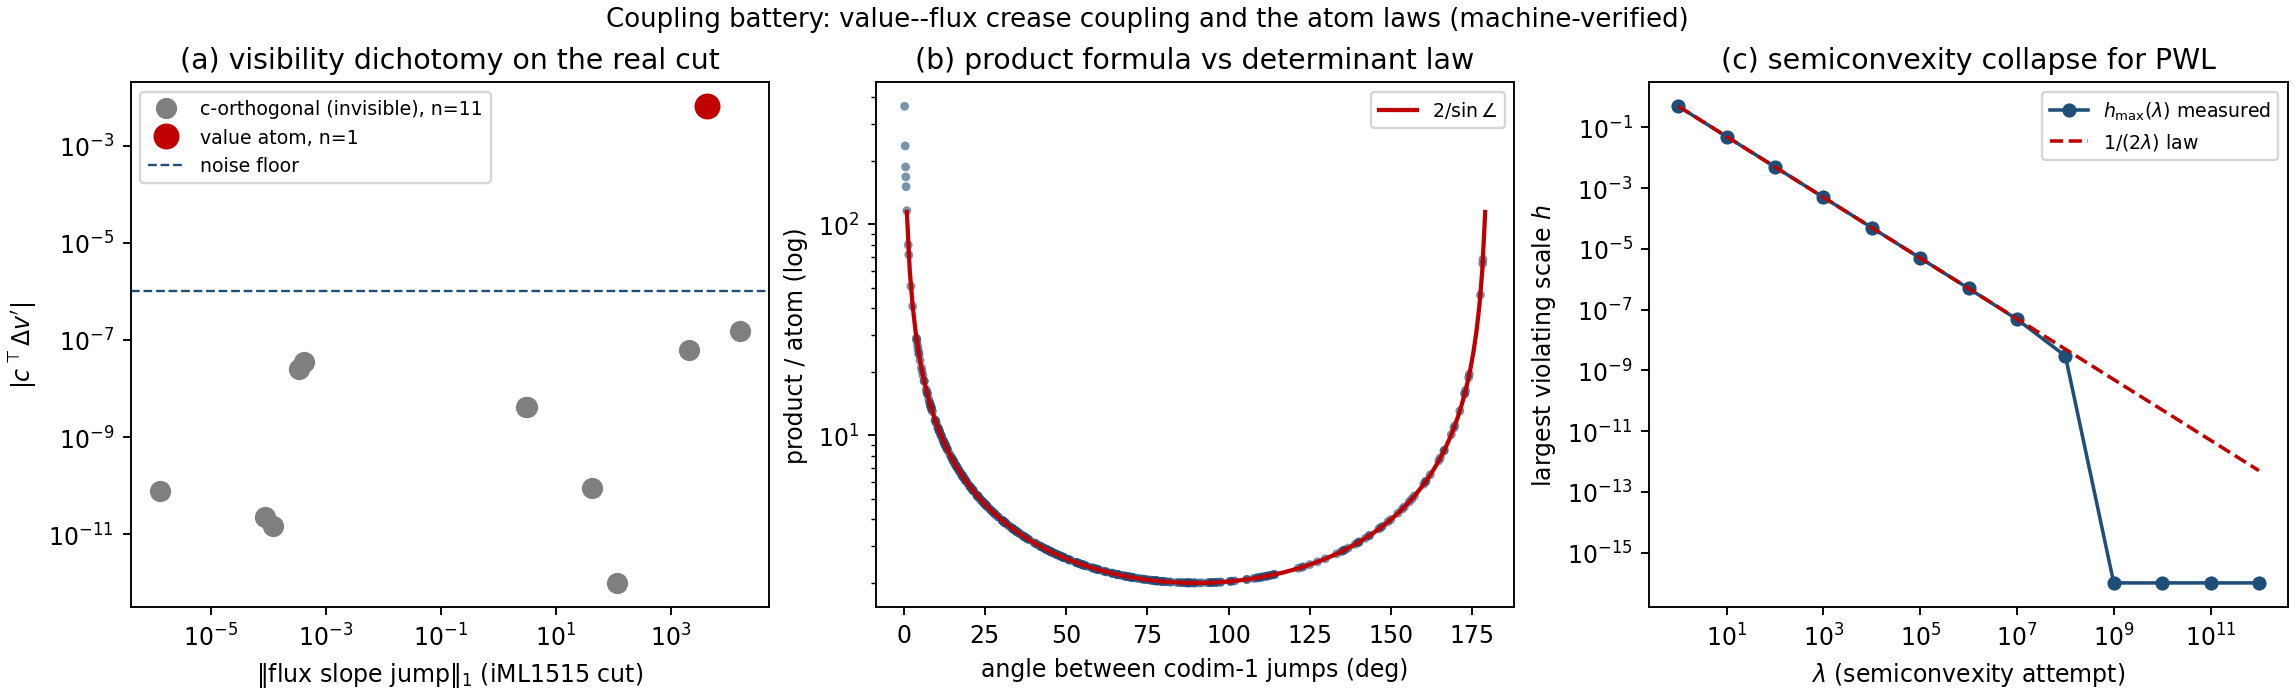
\includegraphics[width=\textwidth]{alexandrov_bridge/coupling_figures.png}
\caption{Machine verification of the value--flux crease coupling (Theorem~\ref{thm:coupling}). The controlled follower-variable LPs:
the value function $\Phi$ stays affine and identical under two
lexicographic tie-breaks while the follower's second-difference mass
flips; the coupling identity $\Delta\Phi' = c^\top \Delta v'$ holds to
$0.0$ on the toys, $1.1 \times 10^{-13}$ on $150$ random dense-objective
LPs, and $2.0 \times 10^{-13}$ on the $60/60$ degenerate follower
family; on the iML1515 cut the identity error is $0.0$ at all $12$
events and all $4$ clusters.}
\label{fig:coupling}
\end{figure}

\subsection{Double-knockout epistasis and path dependence}
Epistasis --- the interaction between two knockouts beyond the sum of
their individual effects --- provides a combinatorial test of the
active-set reading: if the measure is a genuine geometry, pairs of
perturbations should interact through it. We test this on $1{,}516$
single knockouts and $2{,}779$ double-knockout pairs across five
panels. Defining epistasis $\varepsilon_{ij} = \kappa_{ij} - \kappa_i -
\kappa_j$, every one of the $40$ synthetic-lethal pairs is an
isozyme redundancy (tktA/tktB, acnA/acnB, metE/metH, \dots) with
pure-emergence epistasis, and $|\varepsilon_{ij}|$ aligns with
active-set footprint overlap (Spearman $\rho_S = 0.865$,
$J_{\mathrm{support}} = 0.800$). Sequential ($L_1$-MOMA
\citep{segre2002}) knockouts open nonzero commutators in $25\%$ of
active pairs, and closed genotype loops fail to return to the initial
state in $66\%$ of pairs --- phenotypic memory, with median holonomy
$\sim 110$.

\subsection{Regime dial}
\label{sec:m4}
The discrete and smooth regimes of Section~\ref{sec:theoremB} can be
separated empirically by setting the loop size $\varepsilon$ against
the smoothing scale $\sigma$ and dialing one against the other --- a
regime dial. The smoothing identity $D^2(v * \phi_\sigma) = (D^2 v) * \phi_\sigma$
holds to kernel self-test error $1.2 \times 10^{-6}$; the measured
crossover $\varepsilon^*/\sigma \in [2.45, 4.11]$ (median $3.1$)
separates the $O(\varepsilon^2)$ smooth regime from the
$O(\varepsilon)$ discrete regime. The scaling slope is $1.00$ on the
interacting stratum, and the regime-dial census resolves the
thin-wedge sliver structure (net measure jump $8.9$ vs.\ nominal
$\pm 1884.6$).

\subsection{The value function as canonical carrier}
\label{sec:v1}
The tie-break-freeness of the value layer
(Proposition~\ref{prop:alex}) is directly testable: solve the same
parametric problem under two different tie-break conventions and
compare layers. $\Phi = c_{\mathrm{bio}}^\top v^*$ is single-valued
with no tie-breaking; it is piecewise affine at $4.2 \times 10^{-13}$
on the flux-event partition, carries one real atom
$\Delta\Phi' = -0.006439$ at $t = 0.0358286$, and decouples from the
flux-jump hierarchy (value/flux mass ratio $1.7 \times 10^{-6}$).
Finite-difference shadow prices match Danskin envelope marginals to
$6$--$7$ digits. A controlled follower-variable LP reproduces the
same structure: the value function stays affine and identical under
two lexicographic tie-breaks while the follower's second-difference
mass flips $0.0100 \leftrightarrow 10^{-13}$ --- the value layer is
canonical (Proposition~\ref{prop:alex}), the flux-strain layer is not
(Corollary~\ref{cor:valueflux}). The coupling identity of
Theorem~\ref{thm:coupling} is machine-verified on this same cut:
$\Delta\Phi' = c^\top \Delta v'$ with error $0.0$ at all $12$
events and all $4$ clusters, $\Phi = c^\top v^*$ to $10^{-9}$, and
the $11$ invisible events carry flux $\ell_1$ slope jumps up to
$1.6 \times 10^{4}$ against $|c^\top \Delta v'| \le 1.51 \times
10^{-7}$ --- the decoupling is the objective contraction, not a loss
of network information.

% =====================================================================
\section{Empirical association and protein-layer buffering}
\label{sec:empirical}

This section takes the metric to data. Which genes does the network
itself flag as rerouting-sensitive, and do those genes respond when
the environment actually tightens? The answer comes in layers: first
a robust transcriptional association, then an explicit negative
result at the protein layer, and finally robustness checks across
trajectories, tie-break conventions, and panels.


\subsection{The gene panel and GPR classes}
\label{sec:e22}
Reaction-based sampling on the reference physiology (glucose $5.0 \to
1.0$, oxygen $22 \to 5$; iJO1366) leaves $438$ of $2{,}583$ reactions
active ($17.0\%$) and $435$ genes with at least one active reaction.
The GPR complexity classes over the active reactions --- single-gene
$254$, isozyme-OR $96$, complex-AND $36$, mixed $18$, no-GPR $34$ ---
are exactly the classes that drive the concavity analysis of
Proposition~\ref{prop:semiconvex}. Four verification checks were
applied to the panel construction. (i) \emph{GPR mapping:} taken from
cobra's authoritative \texttt{reaction.genes}, spot-checked against
the raw rule strings on four reactions spanning all complexity
classes, with set-equality of gene tokens and a bidirectional
gene--reaction symmetry check on $50$ sampled genes ($0$ failures over $120$
gene--reaction pairs). (ii) \emph{Definition consistency:}
the fresh re-derivation reproduces the deposited values exactly
(per-gene maxima, the biomass-deficit maximum, and the
unmasked/masked panel correlations to four decimals). (iii)
\emph{Distinctness:} the panel shares exactly one b-number with the
$\kk$ panel ($b2097$). (iv) \emph{Non-zero variation:} every panel
gene has $\kappa_V$ variation $> 0$ over T1--T8 ($435/435$). For
completeness, the geometric metric $\kk$ is weak at the panel level
($r$ from $-0.063$ unmasked to $+0.084$ masked); the
measure-theoretic $\kmu$ (\S\ref{sec:v5}) is the recalibrated predictor
on the same panel.

\subsection{Multi-condition support}
\label{sec:e23}
Nine FBA conditions were probed (baseline carbon decline; galactose,
trehalose, glycerol-3-P, and proline-N carbon sources;
anaerobic-nitrate, oxidative, and osmotic designs): active-reaction
support is $438$--$454$ per condition, with union $537$ ($20.8\%$),
and genes with nonzero $\kk$ expand $435 \to 525$ across
conditions. The endogeneity check is clean (feed caps non-binding
except the designed glycerol-3-P limitation; imposed-burden
magnitudes flagged as not interpretable). The rerouting metric is
thus well posed across carbon sources and stress designs: its support
\emph{expands} with condition diversity rather than migrating --- the
measure sees more of the network as the environment demands more of
it.

\subsection{Transcriptional response under carbon depletion}
\label{sec:v5}
On the deterministic lexicographic trajectory (the reference physiology, iJO1366),
we compare $\kmu$ (Definition~\ref{def:kmu}) against log-fold
carbon-depletion response (M3D \citep{faith2008}, $n = 424$ genes;
Fig~\ref{fig:v5}). The association is present and strong: Pearson
$r = +0.395$ ($p = 2.6 \times 10^{-17}$), Spearman
$\rho_S = +0.414$ (full panel, zeros included). One confound
deserves a direct look: because highly expressed metabolic enzymes
often show broader regulatory dynamic ranges, the raw association
could partly reflect baseline expression rather than rerouting.
Residualizing the M3D reference level leaves the association intact
(partial $r = +0.269$, $p = 1.8 \times 10^{-8}$), and the extreme
deciles separate cleanly (top versus bottom response $1.92$ vs
$0.89$; MWU $1.3 \times 10^{-7}$). The baseline reproduces to the
digit ($r = +0.3739$, $n = 433$), and metric invariance holds,
$\rho(\kmu, \kk^{\mathrm{lex}}) = 0.99998$: both metrics sample the
same flux-event structure along the same lexicographic trajectory,
so the association is an event-structure property of the flux layer ---
not a metric artifact and not a value-function shadow. A
cross-platform replication with the declared metric completes the
picture. The carbon-switch arms replicate on the same platform (M3D
microarray: glycerol $+0.195$, acetate $+0.166$, proline $+0.175$,
switch-MAX $+0.206$; $n = 424$ genes, all $p < 6 \times 10^{-4}$)
but dissociate across platforms --- the PRECISE RNA-seq
carbon-switch statistic (ten WT non-glucose carbon conditions)
gives $r = -0.044$ (partial $-0.088$, NS), with individual
conditions weakly positive (glycerol $+0.126$, acetate $+0.130$,
fructose $+0.099$) except galactose ($-0.088$). The association is
thus specific to the carbon-exhaustion class and the platform-matched
design; the cross-platform dissociation is reported as a negative
result.

\subsection{The layer decision}
\label{sec:v6}
Which layer carries the association? We answer this by running every
value-layer attribution arm under the declared protocol of \S\ref{sec:v5}
(iJO1366, the reference physiology, $n = 424$ genes). The flux layer
$\kmu$ gives $r = +0.395$,
partial $r = +0.269$ ($p = 1.8 \times 10^{-8}$); the $c$-attribution
arm is supported on the biomass pseudo-reaction alone ($0$ of $433$
genes; Theorem~\ref{thm:coupling}(ii)); the shadow-price-jump arm
gives $51$ genes at $r = +0.032$ (partial $-0.013$, $p = 0.93$). The
value trajectory has \emph{zero} chamber crossings: the path stays in
one chamber of $\Phi$ throughout --- $\Phi$ is affine along it, with
$d\mu/dq_{\mathrm{glc}} = Y = 0.099544$ ($= |y_{\mathrm{glc}}|$, the
constant glucose uptake shadow price; affine intercept $-0.0124$) and
uptake shadow prices jumping by exactly zero --- all four value kinks
are anchor corners of the trajectory design, of magnitude
$Y\,\Delta(dq_{\mathrm{glc}}/dt)$, carrying no network structure. Value/flux strain mass ratio
$1.45 \times 10^{-3}$; the coupling identity holds at machine
precision (error $0.0$ at every kink). The value-gated flux strain
coincides with $\kmu$ exactly ($433/433$ genes attain their maximum
at a value-kink time), a property of the trajectory design (anchor
rerouting dominates per-gene maxima), not evidence of value-layer
content. The layer decision: the association lives on the flux layer,
with Theorem~\ref{thm:coupling} as the exact bridge to the canonical
object.

\subsection{Path robustness: what survives a trajectory change}
\label{sec:v7}
Three trajectories through the same LP (same engine, seed, panel, statistics; only the path and its matched response vary; Fig~\ref{fig:v7}): P0 glucose decline (reference-physiology anchors; the layer-decision control of \S\ref{sec:v6}), P1 oxygen limitation
($q_{\mathrm{glc}} = 5$ fixed, $q_{O_2}$ linear from $22$ to $1$),
P2 acetate switch ($q_{O_2} = 22$ fixed; glucose $5 \to 0$ while
acetate uptake ramps $0 \to 10$). Kinks are classified by the
chamber test --- the parameters are the uptake bounds, so
$\nabla\Phi = (y_{\mathrm{glc}}, y_{O_2}, y_{\mathrm{ac}})$: a kink is
a \emph{design corner} iff it sits at a trajectory anchor and the
uptake shadow prices are continuous across it (jump $\le 10^{-9}$),
and a \emph{chamber crossing} iff they jump.
\begin{enumerate}[label=(\roman*),leftmargin=2em]
\item The one-chamber property is \emph{path-dependent}: P0 has zero
      chamber crossings (the \S\ref{sec:v6} control, reproduced digit-exactly), while P1 has
      three genuine crossings ($q_{O_2} \approx 9.3$, $6.3$, $2.9$;
      $|\Delta\Phi'|$ up to $0.68$; $y_{O_2}$ jumps $+0.032$ at the
      respiratory boundary) and P2 has four (two large, near the
      glucose--acetate handoff; two micro-slivers with dual jumps
      $\sim 10^{-4}$). The single-chamber structure of the reference trajectory is a property of the glucose-decline design, not a law.
\item The layer decision survives the change: on every path the
      value-layer arms contribute nothing. The $c$-attribution arm is
      degenerate ($0$ of $433$ genes --- the sparse-objective
      corollary of Theorem~\ref{thm:coupling} is path-free); the
      chamber-crossing shadow-price arm is null ($r = -0.17$,
      $n = 68$ on P1; $r = +0.032$, $n = 71$ on P2); value-gated flux
      strain is a subset of $\kmu$ (equal or weaker on every path,
      never stronger).
\item The flux-layer association generalizes: against the matched
      oxygen response (M3D WT anaerobic vs aerobic contrast) P1 gives
      $r = +0.318$ (partial $+0.258$, $p = 6 \times 10^{-8}$,
      $n = 426$); against the matched acetate-switch response P2
      gives $r = +0.223$ (partial $+0.160$, $p = 9 \times
      10^{-4}$); and the P1/P2 predictors correlate with the primary-panel carbon response at $r = +0.378$ / $+0.391$ --- the per-gene
      ranking is largely trajectory-independent.
\item Theorem~\ref{thm:coupling} holds at every kink on all three
      paths (identity error $0$; worst case $1.6 \times 10^{-15}$).
      Value/flux strain mass ratios: $1.5 \times 10^{-3}$ (P0),
      $2.4 \times 10^{-4}$ (P1), $5.5 \times 10^{-4}$ (P2).
\end{enumerate}

\subsection{Tie-break robustness: the association as a property
of the protocol class}\label{sec:v8}

The flux layer is selection-dependent by construction
(Remark~\ref{rem:lock}); the declared lexicographic tie-break is one
member of a family. The tie-break experiment fixes the entire protocol of the primary association (iJO1366, reference-physiology anchors, $8\times$ refinement, the $433$-gene panel, the M3D carbon-depletion response, the reference-level confound control) and varies \emph{only} the stage-3 tie-break of the
engine:
\begin{itemize}
\item \textbf{TB0} (declared): $w \sim U(0.5, 1.5)$, seed 20240901,
      $\min w^\top v$ --- the declared metric (control: reproduces the
      primary association, $r = +0.3954$, digit-exactly);
\item \textbf{TB1} (fresh seed): $w \sim U(0.5, 1.5)$, seed 20240902
      --- same family, independent draw;
\item \textbf{TB2} (family swap): $w \sim \mathrm{LogN}(0, 1)$ clipped
      to $[0.05, 20]$, seed 20240903 --- a different distribution
      family with a roughly $130$-fold wider dynamic range
      (support ratio $400{:}1$ versus $3{:}1$);
\item \textbf{TB3} (rule swap): stage-3 objective on the split
      variables, $\min \sum_r w_r (f_r + r_r)$ --- weighted
      \emph{absolute}-flux selection with TB0's weights;
\item \textbf{TB4} (adversarial): $\max w^\top v$ --- the far end of
      the stage-2-pinned optimal face, with TB0's weights.
\end{itemize}

\begin{table}[t]
\centering
\caption{Tie-break robustness of the association (primary protocol fixed; only the stage-3 selection rule varies). The value layer
(stage-1 biomass $\mu$) and the pFBA layer (stage-2 $\ell_1$, $s_2$)
are invariant to $0.0$ across all variants --- the measured form of
the tie-break-freeness of Proposition~\ref{prop:alex}.}
\label{tab:v8}
\begin{tabular}{lccccc}
\toprule
Variant & $n_{\mathrm{nz}}$ & $r$ & partial $r$ &
$\rho_S(\kmu, \kmu_{\mathrm{TB0}})$ & genes changed \\
\midrule
TB0 declared       & 424 & $+0.3954$ & $+0.269$ & --- & --- \\
TB1 fresh seed     & 426 & $+0.3861$ & $+0.270$ & $0.99998$ & 91 \\
TB2 LogN family    & 424 & $+0.3954$ & $+0.269$ & $0.99999$ & 90 \\
TB3 $|v|$ rule     & 425 & $+0.3959$ & $+0.269$ & $0.99897$ & 109 \\
TB4 $\max w^\top v$& 424 & $+0.3954$ & $+0.269$ & $0.99998$ & 117 \\
\bottomrule
\end{tabular}
\end{table}

Three findings (Table~\ref{tab:v8}, Fig~\ref{fig:v8}). (i) \emph{The association is
stable:} across all five rules $r \in [+0.386, +0.396]$ (maximum
deviation $0.009$; all $p \le 1.4 \times 10^{-16}$) and the partial
correlation is constant to three decimals ($+0.269$--$+0.270$). (ii)
\emph{The tie-break genuinely binds:} the stage-2-pinned optimal face
is multi-vertex, and the alternative rules select different flux
vectors at all $57$ grid points (max $\|v_k - v_0\|_\infty$ up to
$5.0$), changing per-gene $\kmu$ for $90$--$117$ of $433$ genes ---
yet the per-gene ranking is essentially unchanged
($\rho_S \ge 0.99897$), and the changed values are small on the
$\kmu$ scale (max absolute change $9.3 \times 10^{-5}$); the TB1
deviation of $0.009$ traces to two boundary genes entering the
nonzero support ($n: 424 \to 426$), not to a reshaping of the metric.
(iii) \emph{The value layer is exactly invariant:} stage-1 biomass
$\mu$ and stage-2 $\ell_1$ mass agree across variants to $0.0$ ---
Proposition~\ref{prop:alex} (tie-break-freeness of the value layer)
measured on the full trajectory. Together with
Corollary~\ref{cor:valueflux} this completes the robustness picture: the
declared selection is a convention, the value layer does not see it,
and the flux-layer association is a property of the lexicographic
protocol class, not of one rule.

\subsection{Event-measure stabilization
(Glivenko--Cantelli type)}\label{sec:e32}

The refinement-stabilization question
(\emph{do the empirical event point measures of the
lex-pFBA map converge as the sampled family grows?}) has a near-term statistical form, executed here on three data sources: random straight cuts through the $(q_{\mathrm{glc}}, q_{O_2})$ signature plane (iML1515, $34\times34$
census, $350$ boundary edges; a pool of $4{,}000$ random cuts
yielding $25{,}107$ cut events), the thirteen parameter sweeps of \S\ref{sec:m1} ($2$ affine, $11$ event-bearing), and the panel protocol of this paper (gene panel and trajectory). The metric is the bounded-Lipschitz
distance (domains normalized to unit diameter, where it equals
$W_1$; exact in one dimension, transport LP in two); each arm carries
a permutation null (event locations replaced by uniforms, panel
structure kept) and the one-dimensional arms carry the classical
Glivenko--Cantelli asymptotic constant
$C = \int\sqrt{F(1-F)}\,dx$ of del~Barrio--Gin\'e--Uzet computed from
the population (Fig~\ref{fig:e32}).
\begin{enumerate}[label=(\roman*),leftmargin=2em]
\item \emph{Random panels stabilize at the GC rate.} Pooled cut-event
      locations on the cut coordinate (d=1): measured tail slope
      $-0.492$ versus null $-0.506$, measured/null ratio $1.24$ at
      the largest panel, and the iid prediction $C/\sqrt{n}$ matches
      the measured curve to $2.5\%$ at the largest panel (mid-range
      deviations as large as $8.2\%$); the two-dimensional pooled
      locations (transport LP) decay consistently with the $d=2$ rate
      up to the reference-noise floor. Sweep panels (the thirteen sweep families) stabilize with a heterogeneity penalty that falls
      from $\approx1.8\times$ the uniform null at small panels
      through $\approx1.5\times$ at $k = 6$ to $\approx0.5\times$ at
      $k = 12$, and a tail faster than iid-GC --- consistent with the
      finite-population correction
      $\sqrt{(13-k)/12}$ of sampling without replacement from
      thirteen heterogeneous sweeps (measured null-relative ratio
      $0.49$ at $k = 12$, against the pure FPC value $0.29$; the
      residual is the sweep heterogeneity). The gene panel: the $\kappa$ distribution stabilizes at the GC rate (measured
      effective constant $\approx 1.6$--$2.1$ across panel sizes
      (dipping at $m = 128$), against the population
      Glivenko--Cantelli constant $C = 2.49$
      on the $\log_{10}\kmu$ axis), and the association itself
      stabilizes at $r \approx +0.39$ with the Fisher standard error
      $1/\sqrt{m-3}$.
\item \emph{Designed panels stabilize exactly, not statistically.}
      The trajectory event point measure is a \emph{four-atom} object: the four design corners of the physiology anchors carry the entire flux-layer mass ($288.77$, the primary association's flux-layer mass to the digit) --- the one-chamber structure of \S\ref{sec:v6} in its event form.
      Anchor-preserving thinning reproduces it \emph{exactly} at every
      panel size $m \ge 8$ (shape distance $0$ to machine precision,
      $\le 7 \times 10^{-13}$; total-mass error $\le 2 \times
      10^{-12}$; value-kink census $\equiv 4$); uniform random
      thinning decays by corner censoring (shape distance
      $0.12 \to 0.005$ by $m = 43$, mass error $26\% \to 0.13\%$ by
      $m = 29$, machine-zero ($\le 3 \times 10^{-12}$) from
      $m = 43$, and exactly $0$ at the full panel $m = 57$) --- a
      resolution effect in the sense of Theorem~\ref{thm:Bprime}(iv),
      not statistical averaging.
\end{enumerate}
Interpretation: the mean-field intuition is confirmed in its
statistical form --- the empirical event measures over random panels
(cuts, sweeps, genes) are Glivenko--Cantelli objects --- and
simultaneously sharpened: stabilization has two regimes, statistical
for random panels and structural (exact, design-immediate) for
designed panels. The deterministic refinement-sequence form of the
question (refinement along explicit model-family sequences) remains open.

\begin{figure}[t]
\centering
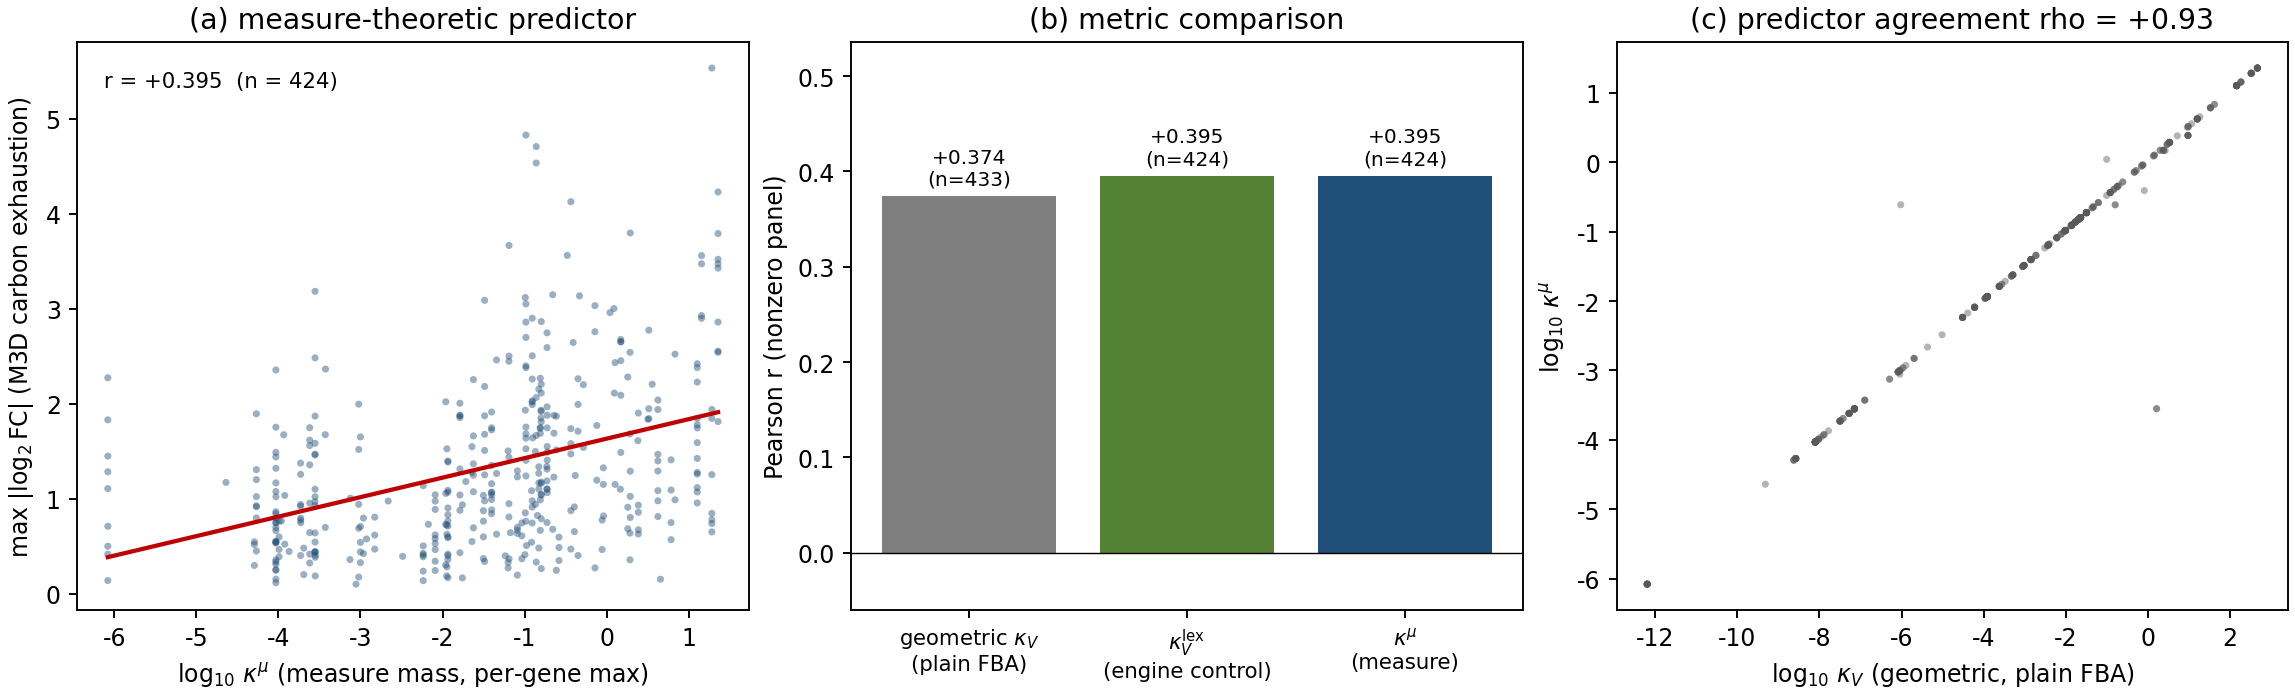
\includegraphics[width=\textwidth]{association_robustness/v5_e24_recalibration.png}
\caption{The primary association. (a) Per-gene
$\log_{10}\kmu$ (flux-layer measure mass, per-gene max over the
gene's reactions) versus M3D carbon-depletion response
($\max|\log_2\mathrm{FC}|$, four stationary contrasts, $n = 424$
nonzero genes); (b) metric comparison: the geometric time-course
$\kk$ (reference physiology, plain-FBA), the engine control $\kk^{\mathrm{lex}}$, and
the measure-theoretic $\kmu$ on the same trajectory; (c) predictor
agreement between $\kmu$ and the plain-FBA $\kk$.}
\label{fig:v5}
\end{figure}

\begin{figure}[t]
\centering
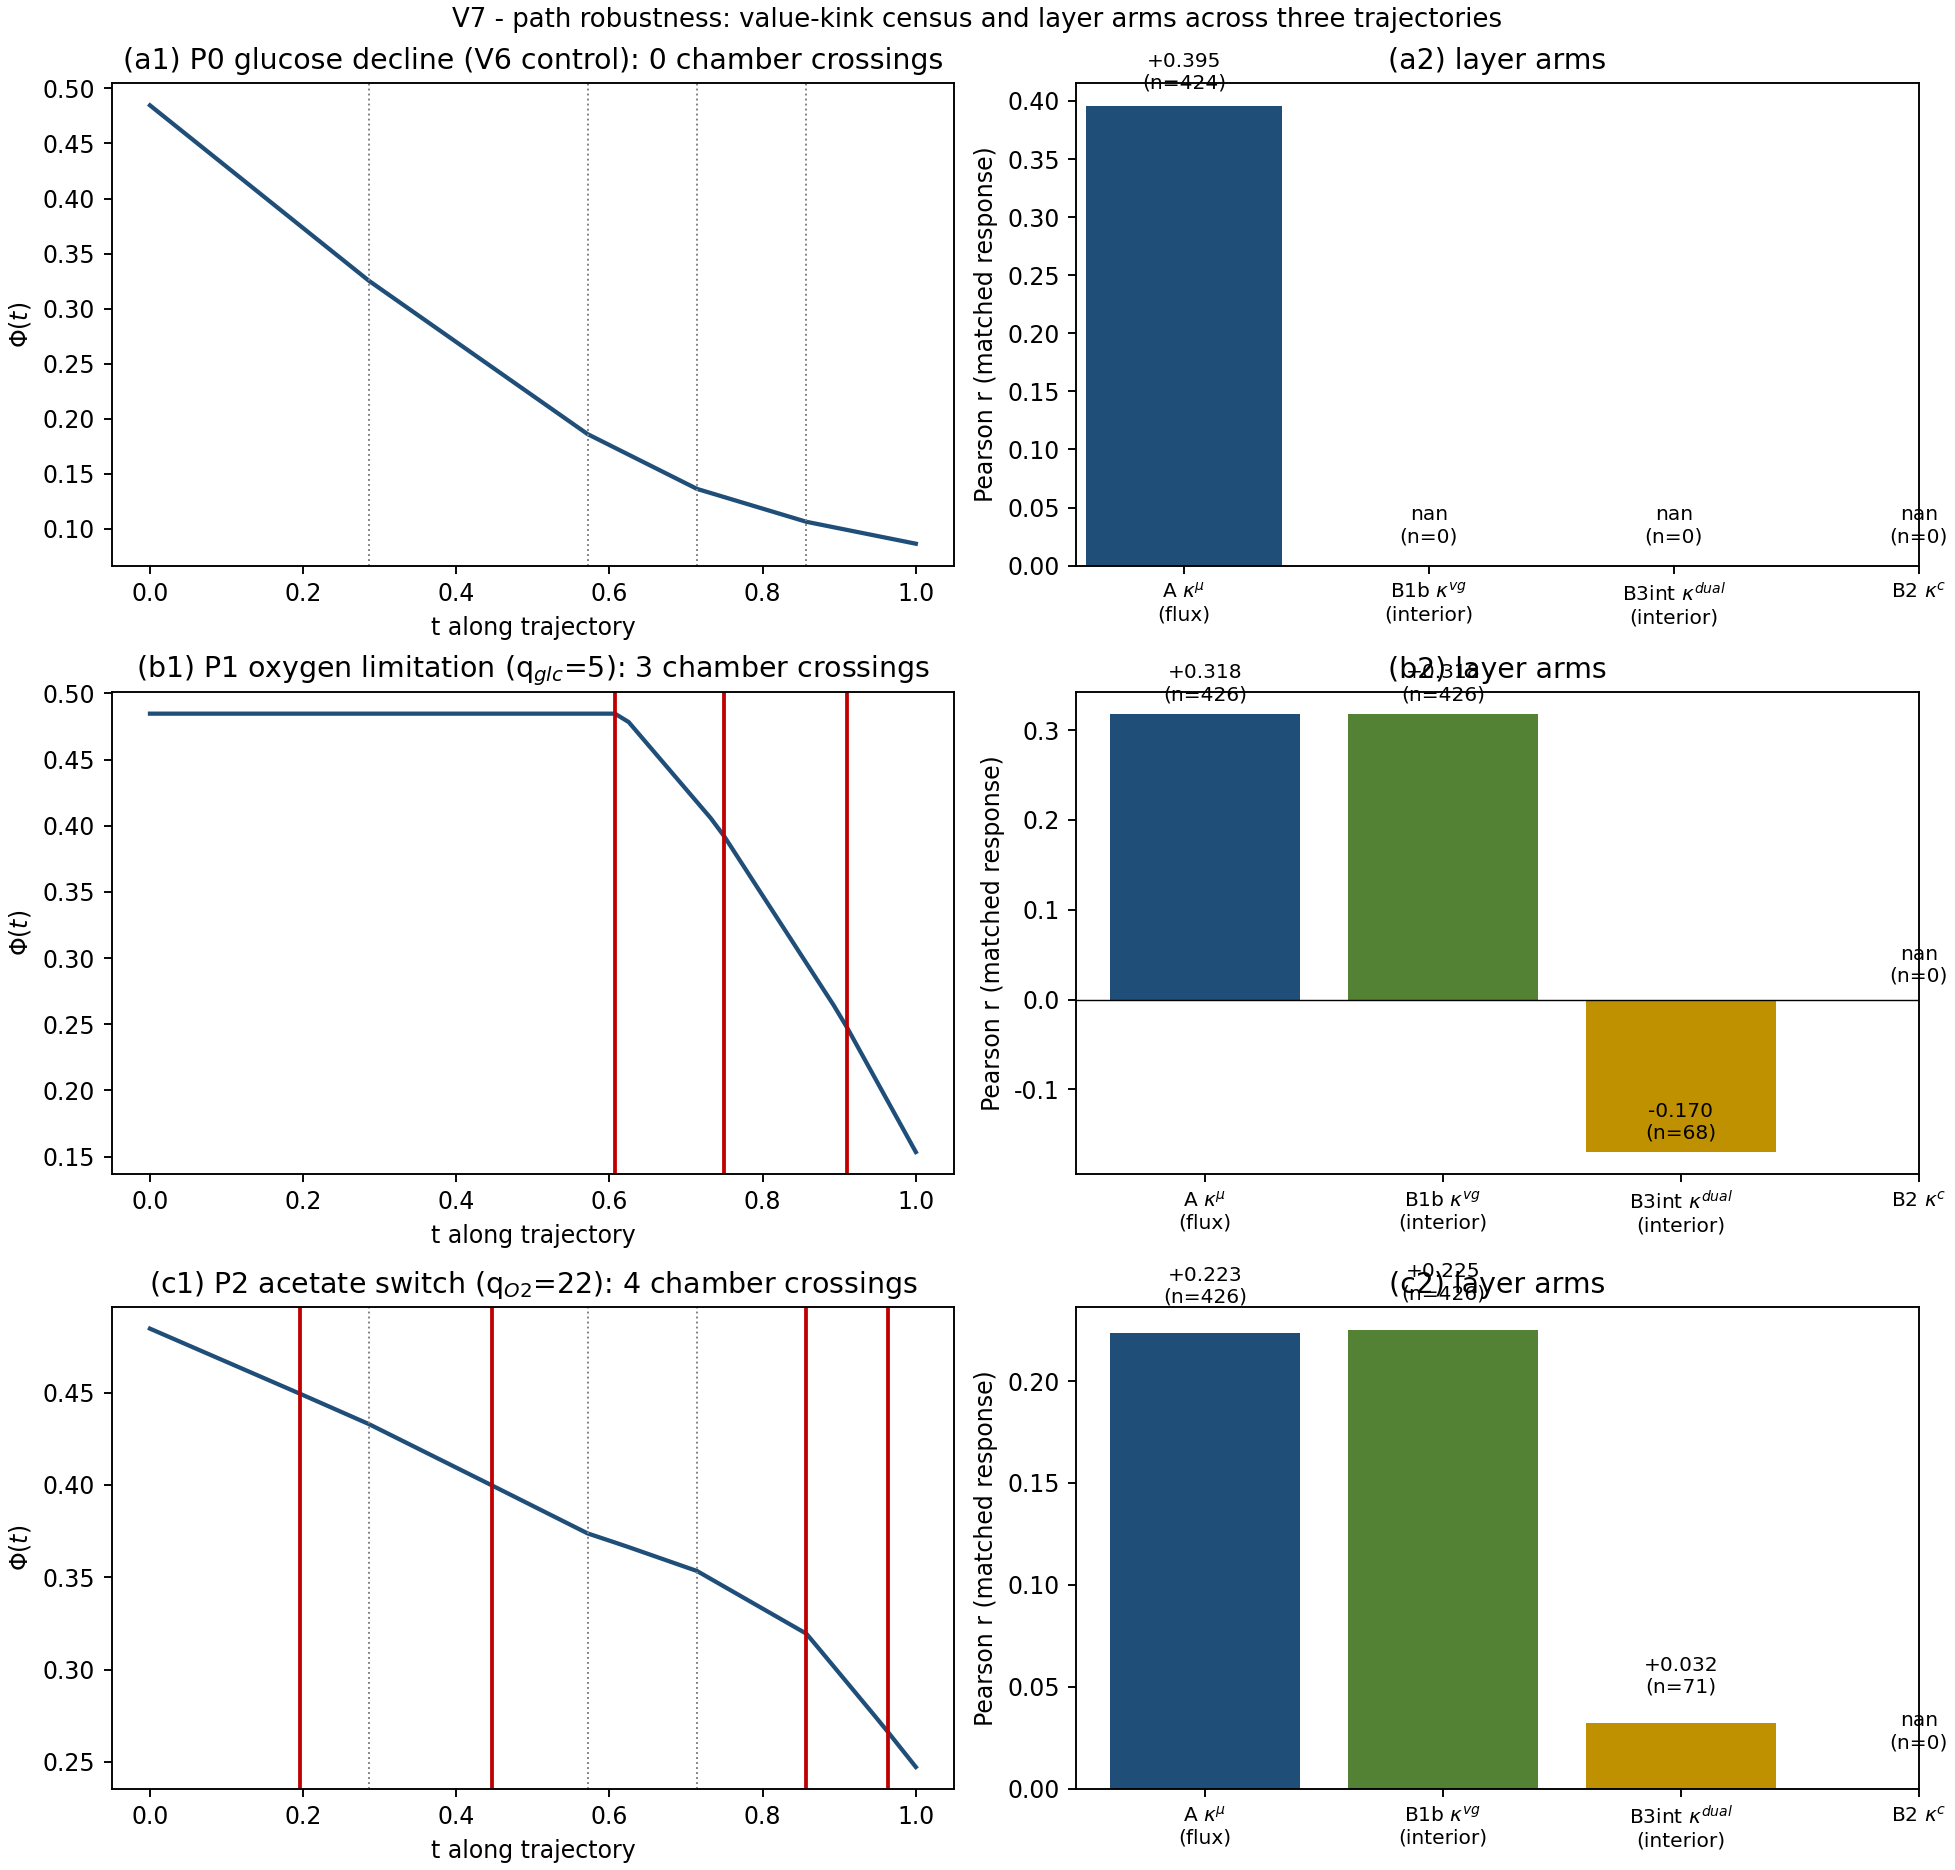
\includegraphics[width=0.86\textwidth]{association_robustness/v7_path_robustness.png}
\caption{Path robustness. Three trajectories through the same
LP (P0 glucose decline, P1 oxygen limitation, P2 acetate switch) with
matched M3D responses: the one-chamber property is path-dependent
(P1: 3 chamber crossings; P2: 4), while the layer decision and the
flux-layer association survive on every path; the P1/P2 predictors correlate with the primary-panel carbon response at $r = +0.378$/$+0.391$.}
\label{fig:v7}
\end{figure}

\begin{figure}[t]
\centering
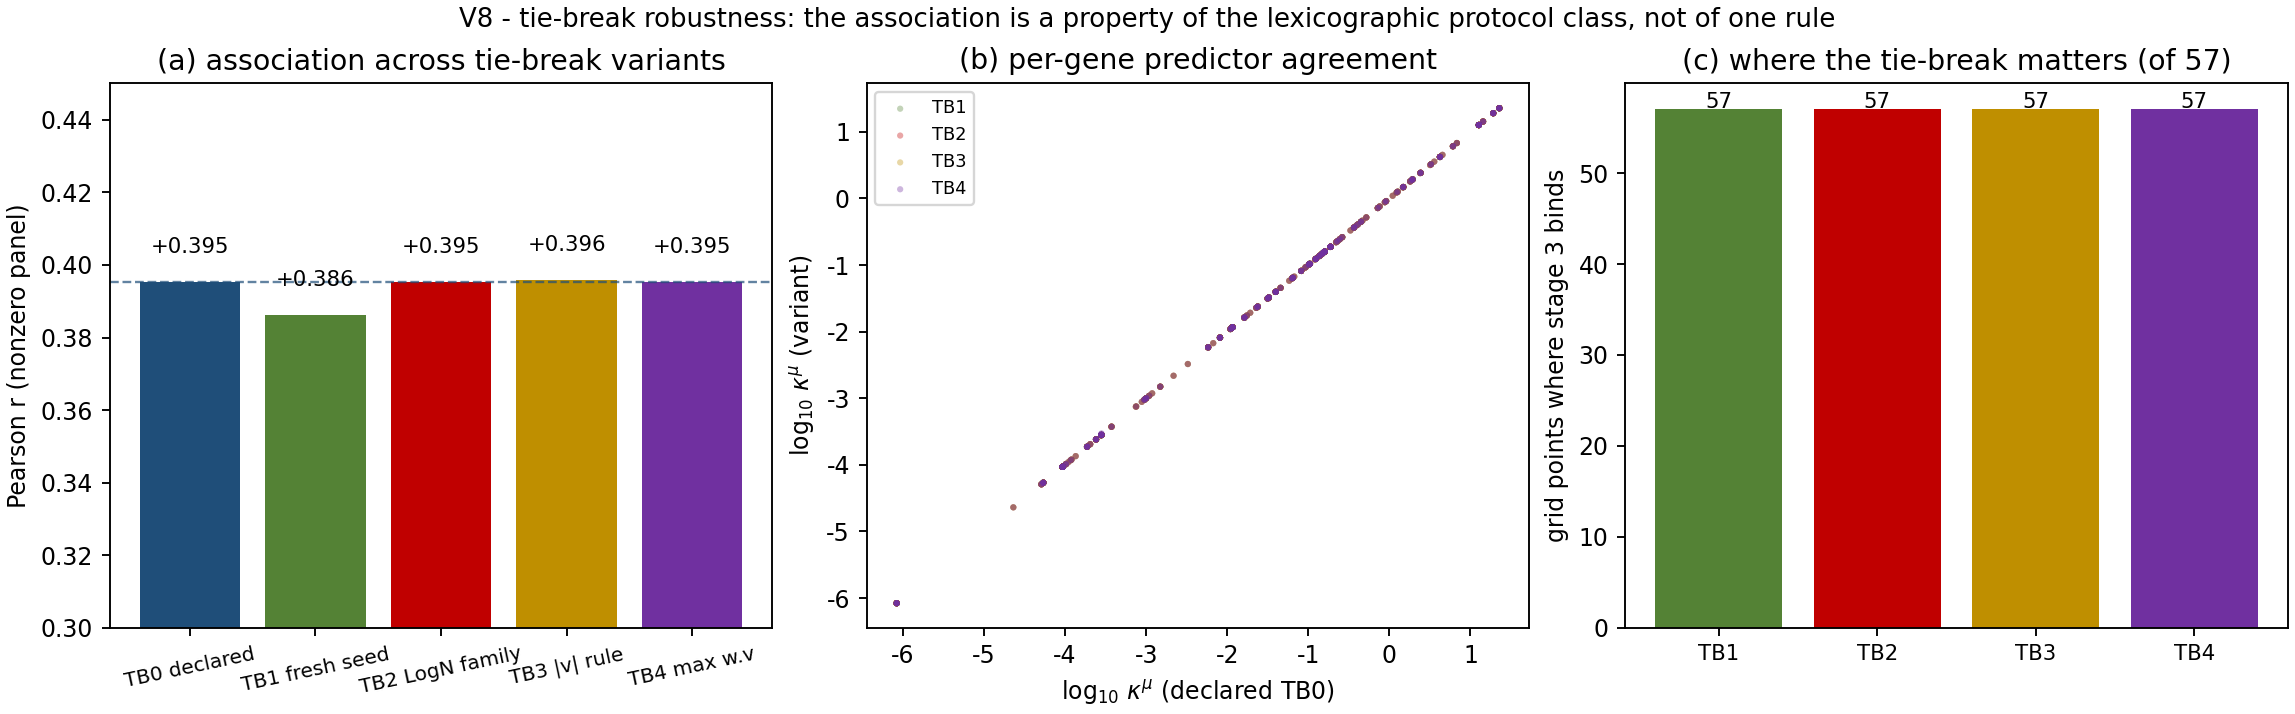
\includegraphics[width=\textwidth]{association_robustness/v8_tiebreak_robustness.png}
\caption{Tie-break robustness. (a) The association across the
five stage-3 selection rules (declared plus four variants); (b)
per-gene predictor agreement between the declared rule and each
variant; (c) the number of grid points at which the tie-break binds (of 57). The value layer is invariant to $0.0$ across all variants.}
\label{fig:v8}
\end{figure}

\begin{figure}[t]
\centering
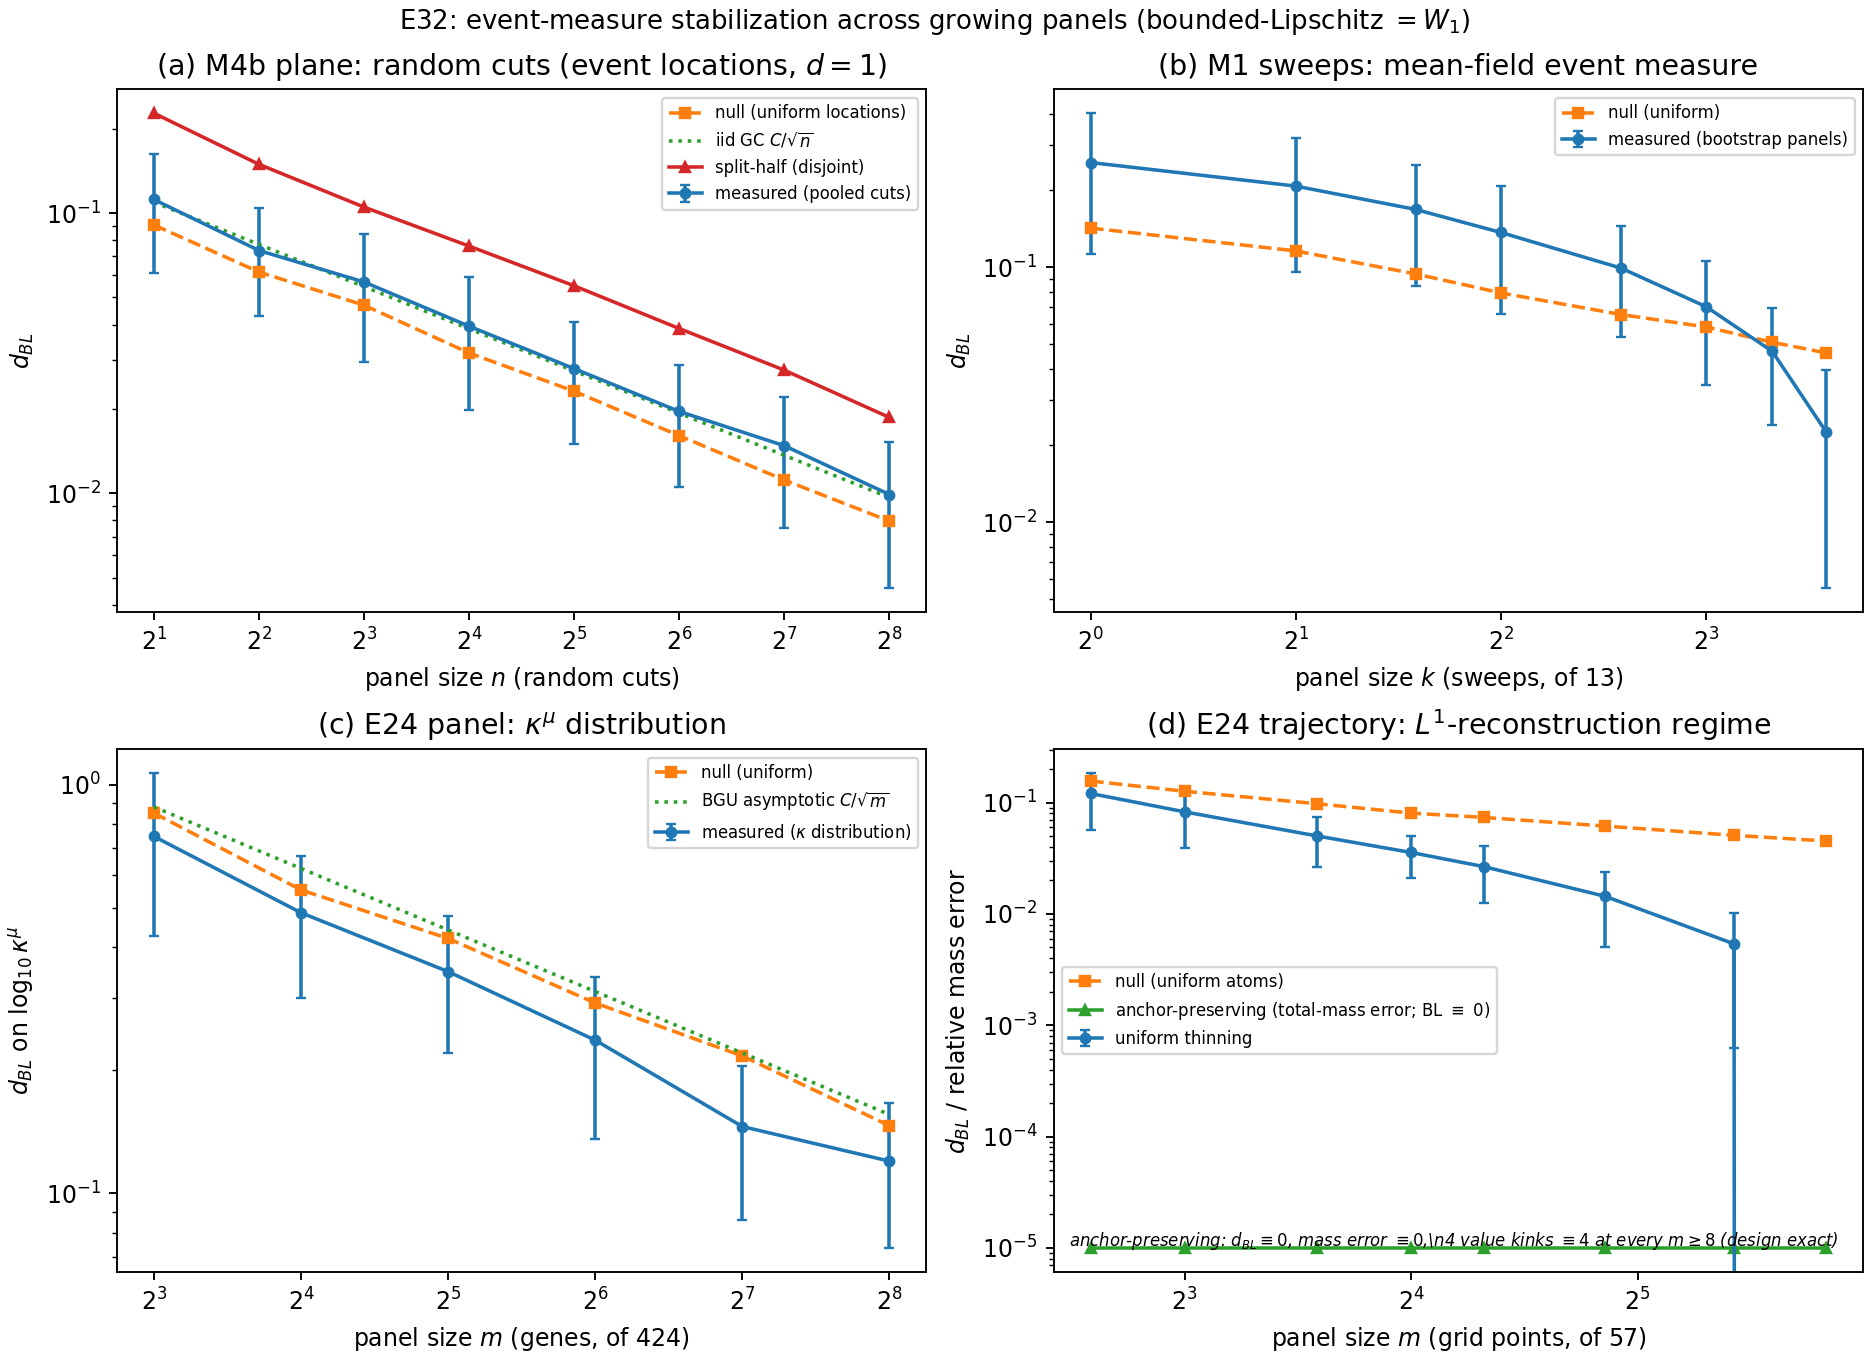
\includegraphics[width=\textwidth]{association_robustness/e32_event_measure_stabilization.png}
\caption{Event-measure stabilization. (a) Random-cut panels:
pooled event-location distance decays at the Glivenko--Cantelli rate
(measured tail slope $-0.492$; null $-0.506$; iid prediction
$C/\sqrt{n}$ to $2.5\%$ at the largest panel, mid-range deviations
as large as $8.2\%$); (b) Parameter-sweep panels: stabilization with a
finite-population-corrected, heterogeneity-penalized tail
(null-relative ratio $0.49$ at $k = 12$ against the pure FPC
$0.29$); (c) Gene panel: the $\kappa$
distribution at the GC rate (effective constant $\approx 1.6$--$2.1$,
dipping at $m = 128$, vs.\ the population constant $C = 2.49$);
(d) Reference trajectory: the $L^1$-reconstruction regime --- random
thinning decays by corner censoring, anchor-preserving thinning is
exact ($d_{BL} \equiv 0$) from $m \ge 8$.}
\label{fig:e32}
\end{figure}

\subsection{Platform-by-class disambiguation ($2 \times 2$)}
\label{sec:e25}
Is the association a carbon-depletion artifact, or a platform
artifact? The question has a clean $2 \times 2$ answer: two platforms
crossed with two perturbation classes, executed with the geometric $\kk$ metric
(rank-equivalent to $\kmu$ at $\rho = 0.99998$). Carbon switch on
microarray (M3D glycerol/acetate/proline vs glucose) switch-MAX $r =
+0.196$; stress on microarray (heat shock, acid shock, ciprofloxacin)
MAX $r = +0.298$; carbohydrate-responsive transcript levels: carbon
starvation on RNA-seq (GSE64021 \citep{barrett2013} time course) MAX
$r = +0.191$; heat shock on RNA-seq MAX $r = +0.345$ ($n = 241$--$433$;
permutation $p \le 0.003$). Signed responses flip sign (stress arms
$-0.22$ to $-0.32$): the metric tracks \emph{rerouting magnitude},
not direction, on both platforms and both classes. The association is
thus neither platform-specific nor carbon-class-specific.

\subsection{Protein abundance versus protein change}
\label{sec:e26}
A central question at this point is whether the transcriptional
association propagates downstream to the proteome. Two dissociations
at the protein layer answer it in the negative (PaxDb integrated
abundance \citep{wang2015}; quantitative proteomics of GSE64021
\citep{barrett2013};
$n = 169$--$429$). First, abundance \emph{level} associates (PaxDb
baseline $r = +0.334$): high-rerouting genes are abundant proteins.
Second, abundance \emph{change} does not (protein log-fold change $r
= +0.008$ to $+0.032$; transcript--protein fold-change coupling
$r = +0.020$, $n = 799$). The transcriptional association thus stops
at translation, consistent with buffering: rerouting capacity is
carried at the transcript level, and the translational cost is
deferred until a rerouting bottleneck actually demands it
(\S\ref{sec:e27}).

\subsection{Protein-layer null}
\label{sec:e27}
The decisive negative result comes from condition-dependent
quantitative proteomics (\citet{schmidt2016}; $22$ conditions, triplicates,
$n = 366$): the protein-level correlation is $r = -0.083$, against
transcript $+0.419$ on the same genes. Strikingly, the association
that is robust at the transcript layer vanishes entirely at the
protein layer. The transcript-level association does not propagate
through translation; buffering at translation is the consistent
model, positioning \citet{kochanowski2013} as prior art for the
protein-layer null.

% =====================================================================
\section{Discussion: one measure, several resolutions}
\label{sec:discussion}

The sensitivity objects of the framework are one measure at different
resolutions: the atomic measure of Definition~\ref{def:mu}, its
coarse-grainings $\mu * \phi_\sigma$, and its integrals along parameter
trajectories ($\kmu$). The smooth member of this family exists only
through the window $h \ll \sigma \ll L_{\mathrm{var}}$; the
$\sigma \to 0$ limit is the atomic object. Outside the window ---
$\sigma$ below the mesh scale or above the variation scale --- the
smooth representation breaks down, and the system is properly
described by its discrete active-set atoms. Two items remain open:
Conjecture~\ref{conj:bridge} (general complex stability) and second
differences on measured time courses (under the $(\varepsilon,
\sigma)$ design law). The statistical form of the stabilization
question is settled here (\S\ref{sec:e32}): random panels are
Glivenko--Cantelli objects and designed panels reproduce the event
measure exactly; the deterministic refinement-sequence form
(refinement along explicit model-family sequences) remains open.
The exact contraction identity
$D^2\Phi = \sum_r c_r\, D^2 v^*_r$ of Theorem~\ref{thm:coupling}
grounds the association's flux-layer footing, complementing the
measured metric invariance of \S\ref{sec:v5}. Because cells routinely
exploit alternative pathways of equal growth during nutrient
transitions, most metabolic rerouting is objective-invisible (the
zero-cost substitutions of Theorem~\ref{thm:coupling}(i)). The
empirical association reflects this separation: gene expression
changes correlate with the flux-layer metric $\kmu$ ($r = +0.395$)
but show no association with value-layer derivatives (shadow-price
arm $r = +0.032$, $p = 0.93$, $n = 51$). Transcriptional response
tracks rerouting, and rerouting is a flux-layer quantity.

\paragraph{Limitations.}
\begin{enumerate}[label=\textbf{\arabic*.},leftmargin=2.2em,itemsep=2pt]
\item \textbf{Design and scope.} The study is correlational by
      design, and its scope is a single organism; whether the
      protein-layer buffering null extends beyond \emph{E.~coli} is
      open.
\item \textbf{Operational active sets.} The active sets used
      throughout are operational (obtained from solved LPs) rather
      than combinatorial.
\item \textbf{Selection dependence.} The lexicographic tie-breaking
      is an engine convention: the value-function carrier is immune
      to it, the flux layer declares it (Remark~\ref{rem:lock}), and
      the association is stable across all five selection rules
      tested (declared plus four variants, \S\ref{sec:v8}).
\item \textbf{Path dependence.} The one-chamber structure of the
      reference path is condition-specific (\S\ref{sec:v7}), while
      the layer decision itself is path-robust.
\item \textbf{Cross-platform generality.} The cross-platform
      carbon-switch dissociation (PRECISE arm, \S\ref{sec:v5})
      bounds the generality of the association.
\item \textbf{Census sensitivity.} The active-reaction census of the
      reference physiology ($438/2{,}583$
      and the GPR class counts) is plain-FBA and solver-version-sensitive
      at the $\pm 1$-reaction level, while the gene-level panel ($435$) is
      stable (Appendix~\ref{sec:counts}).
\item \textbf{Stabilization limits.} The sweep arm of the
      stabilization experiment is panel-limited (thirteen sweep
      families, two of them affine --- the finite-population
      correction is part of the reported result), and the
      two-dimensional arm is floor-limited at large panels by the
      transport-LP atom cap.
\end{enumerate}

\paragraph{The companion theory paper.}
The categorical and homotopy-theoretic reading behind the
active-set curvature interpretation --- the $2$-category
$\mathbf{StCon}(B)$ of stratified connections with its gluing
theorem, the Fisher-minimal transport law on constant-active-set
strata, the optic-composition semantics with its contraction
analysis, the filtered-colimit construction of autocatalytic sets,
the viability-kernel reading of its dynamical closure test (a
finite-time, feedback-certifying probe of kernel and capture-basin
membership, with the Poincar\'e/averaging analysis of its pathwise
levels), and the homotopy-type-theoretic extension --- is developed
in full,
as a standalone theory paper with its own proofs, machine
verifications, and per-result proof-status marking (the
homotopy-type-theoretic extension is proof-sketch-marked there; the
stratified gluing is descent-by-citation with construction-level
verification), in a companion manuscript \citep{zai2026categorical}.
The division of labor is deliberate: this paper is the application --- the
measure-theoretic curvature of parametric FBA, the metric $\kmu$,
and the genome-scale empirical association with its layer decision
--- and carries only a brief adapted statement of the load-bearing
definitions (\S\ref{sec:categorical}); the companion carries the
framework. Neither manuscript depends on the other's claims.

\paragraph{Scope of the contribution.}
The mathematics is classical: parametric linear programming (chamber
complexes, active sets, Danskin duality \citep{danskin1967}), Alexandrov's theorem \citep{alexandrov1939}, and
distributional second derivatives of piecewise-affine maps;
Theorem~\ref{thm:coupling} is an elementary identity. The contribution
is the systematic \emph{application} of this machinery to flux-balance
models \citep{varma1994, orth2010, lewis2010} --- the two-layer measure structure of the value/flux pair,
the exact coupling identity, the signed extension to arbitrary GPR
structure --- together with the empirical association and its layer
decision. No new measure-theoretic theorem is claimed; the nearest
prior art (phenotype phase planes \citep{edwards2001, ibarra2002}, mpLP
value-function theory \citep{borrelli2003},
discrete Monge--Amp\`ere \citep{gutierrez2001}, Regge-type defect measures \citep{regge1961, cheeger1984}) is cited where
it applies.

% =====================================================================
\section{Methods}\label{sec:methods}


\subsection{The lexicographic pFBA engine}\label{sec:engine}

All deterministic trajectories are computed by a purpose-built
three-stage lexicographic solver --- the engine that makes every
preceding experiment reproducible --- on the variable split $x = (v, f,
r)$ with $v = f - r$, $f, r \ge 0$, stoichiometry $Sv = 0$, and
flux bounds $\ell(\theta) \le v \le u(\theta)$ entering affinely
through the uptake bounds. The stages are strict lexicographic
optimizations, each pinned at the previous stage's optimum:
\begin{align}
\text{(1)}\quad & \mu^* = \max\; c_{\mathrm{bio}}^\top v
  \qquad\qquad\qquad\qquad\quad\; \text{(growth)} \notag\\
\text{(2)}\quad & s^2 = \min\; \textstyle\sum_r (f_r + r_r)
  \quad\text{s.t. } v_{\mathrm{bio}} \ge \mu^*(1 - \varepsilon_\mu)
  \qquad \text{(parsimony)} \notag\\
\text{(3)}\quad & \min\; w^\top v
  \quad\text{s.t. } \textstyle\sum_r (f_r + r_r) \le s^2(1 +
  \varepsilon_s) \qquad \text{(tie-break)} \notag
\end{align}
with $\varepsilon_\mu = \varepsilon_s = 10^{-9}$ and $w \sim U(0.5, 1.5)$ drawn once with seed 20240901 and fixed thereafter.
Stage 3 exists for a reason: plain pFBA is vertex-degenerate on these
models, with repeated warm-started solves of the same LP flipping
$0.69$ reactions on average between vertices of the optimal face. The
LPs are solved with HiGHS
\citep{huangfu2018} via \texttt{scipy.optimize.linprog}, cold-started
and deterministic; a presolve-disabled retry handles the rare
infeasibility mis-report. The lex optimum exists, is unique by
construction, and is continuous piecewise affine in $\theta$
(Lemma~\ref{lem:lex}); the tie-break is part of the metric's
definition (Remark~\ref{rem:lock}), and its robustness is measured in \S\ref{sec:v8}. The active-reaction census of the reference physiology is the one plain-FBA computation retained (kept for comparability with the geometric metric $\kk$); it is solver-version-sensitive at the $\pm 1$-reaction
level, while the gene-level panel is stable.

\subsection{Models and data provenance}\label{sec:data}

\paragraph{Models.} \emph{E.~coli} iJO1366 (2{,}583 reactions) \citep{orth2011} for the association experiments of \S\ref{sec:empirical}; iML1515 \citep{monk2017} for the computational batteries of \S\ref{sec:computational} and the value--flux coupling verification cut. Genome-scale models are
loaded from the local BiGG JSON copies with SHA-256 manifests.

\paragraph{M3D microarray compendium.} The expression panels come from
the M3D \emph{E.~coli} compendium v4 Build 6
\citep{faith2008, faith2007}: 4{,}297 gene probes $\times$ 907
arrays, log$_2$ uniformly normalized. The carbon-depletion response
is the maximum $|\log_2\mathrm{FC}|$ over the four stationary
time points (135/330/480/720 min) against the MOPS glucose
reference; the oxygen-limitation and acetate-switch responses use
the M9 WT anaerobic versus aerobic and MOPS acetate versus glucose
contrasts. The reference-level confound control is the mean
log-phase WT MOPS glucose expression. The 117~MB compendium
tarball is not committed (repository size); it is re-downloadable
from the recorded URL with the committed SHA-256
(\texttt{e73088f7\allowbreak\ldots}).

\paragraph{PRECISE.} The cross-platform arm uses the ten WT
non-glucose carbon conditions of the PRECISE compendium
\citep{sastry2019} (RNA-seq, TPM). PRECISE has no carbon-depletion class; the dissociation is reported as a negative result with per-condition values (\S\ref{sec:v5}).

\paragraph{Proteomics.} Condition-dependent quantitative proteomics
from \citet{schmidt2016} (22 conditions, triplicates); integrated
protein abundance from PaxDb \citep{wang2015}; the GSE64021
\citep{barrett2013} time course supplies the RNA-seq
carbon-starvation and the quantitative proteomics arms (\S\S\ref{sec:e25}--\ref{sec:e26}).

\subsection{Panel construction and GPR association}

The gene panel is built by reaction-based sampling: solve the lexicographic trajectory on the reference physiology (glucose $5.0 \to
1.0$, oxygen $22 \to 5$; eight anchors, $8\times$ per-segment
trajectory refinement), take the $438$ reactions active
($|v| > 10^{-9}$ at any grid point) on the plain-FBA census of the
reference physiology,
classify each active reaction's GPR rule (single-gene $254$,
isozyme-OR $96$, complex-AND $36$, mixed $18$, no-GPR $34$), and
assign each gene the maximum over its associated reactions. The expression panel consists of the $433$ genes of this set carrying M3D response
data; the primary correlation uses the $424$ genes with nonzero
$\kmu$. The near-colliding gene/reaction counts
($424/433/435/438/440/525/537$) are disambiguated in Appendix~\ref{sec:counts}.

\subsection{Statistical protocols}

The predictor is $\log_{10}$ of the per-gene $\kmu$ (its
distribution is log-linear over five decades); the response is
$\max|\log_2 \mathrm{FC}|$ of the matched contrast. Reported
statistics: Pearson $r$ with analytic $p$, Spearman $\rho_S$
(raw predictor ranks, full panel and nonzero subset as labeled),
partial $r$ controlling the M3D reference level by linear
residualization of both variables, permutation $p$ ($10^5$
label permutations, Monte Carlo), bootstrap 95\% CIs ($10^4$
resamples), and top-vs-bottom decile contrasts (one-sided
Mann--Whitney $U$). All tests are two-sided except the decile
contrast. The PRECISE per-condition arms use the same protocol
with TPM log-fold changes. Every manuscript number traces to a deposited artifact file and is re-derived by the automated numeric verification described under Reproducibility ($301$ checks).

\subsection{Reproducibility}

All experiments deposit their result files and generating
scripts in the public repository cited in the Data Availability
statement. Independent-seed reproductions are recorded for the
refinement prototype and the stress batteries. The layer-decision,
path-robustness, and tie-break-robustness analyses, the cross-platform
arm, and the event-measure stabilization re-run in minutes each on a
single workstation. An automated suite of $301$ numeric checks
re-derives every manuscript number from the deposited artifacts and
is re-runnable end-to-end.

% =====================================================================
\appendix
\section{Disambiguation of near-colliding counts}\label{sec:counts}

Near-colliding counts in the manuscript, each traceable to a single deposited artifact file (Data Availability):

\noindent\begin{minipage}{\textwidth}\footnotesize
\begin{tabularx}{\textwidth}{@{}l>{\raggedright\arraybackslash}X@{}}
\toprule
\textbf{Value} & \textbf{Meaning (source)} \\
\midrule
$2{,}583$ & iJO1366 reactions (model file; recomputed) \\
$438$ & reactions active on the reference physiology, $17.0\%$ (plain-FBA census, $\pm 1$ solver sensitivity) \\
$440$ & reactions with $D_2 > 10^{-8}$ along the reference trajectory (reaction-level event count, deposited event file) \\
$433$ & panel genes with M3D response (panel file row count) \\
$424$ & panel genes with nonzero $\kmu$ --- the $n$ of the primary correlation (deposited metric file) \\
$426$ & nonzero genes on the P1/P2 paths (deposited path file) \\
$435$ & genes with $\ge 1$ active reaction, reference physiology (census file; recomputed exactly) \\
$454$ & max active reactions across the nine multi-condition panels (deposited multi-condition results) \\
$537$ & union of active reactions across conditions, $20.8\%$ (deposited multi-condition results) \\
$525$ & genes with nonzero $\kappa$ across conditions (deposited multi-condition results) \\
$4$ & trajectory atoms of the event measure --- the four design corners carrying the full flux-layer mass $288.77$; identical to the value-kink positions (deposited event files) \\
$350$ & boundary edges of the $(q_{\mathrm{glc}}, q_{O_2})$ signature census, full $34\times34$ grid (deposited census grid) \\
$25{,}107$ & cut events in the random-cut pool, $4{,}000$ cuts (stabilization artifact) \\
$1{,}516$ & iML1515 genes, single knockouts (deposited knockout file) \\
$2{,}779$ & double-knockout pairs, five panels (deposited knockout file) \\
\bottomrule
\end{tabularx}
\end{minipage}

\section{Proofs}\label{sec:proofs}

This appendix proves the results of the manuscript in full. Where an
argument would repeat textbook material, the standard source is cited
in lieu of reproduction; the two long technical arguments
(Lemma~\ref{lem:lex} and the reconstruction part (iv) of
Theorem~\ref{thm:Bprime}) are delegated to
Appendix~\ref{sec:techproofs} and cited there.

\subsection{Proof of Proposition~\ref{prop:alex}}

Write the primal as $\max\{c^\top v : Sv = 0,\ \ell(\theta) \le v
\le u(\theta)\}$ with $\ell, u$ affine in $\theta$. Its dual is
\[
\min\ \bigl\{u(\theta)^\top w^{+} - \ell(\theta)^\top w^{-}
\;:\; S^\top y + w^{+} - w^{-} = c,\; w^{\pm} \ge 0\bigr\},
\]
with $y$ free. The constraint set $\mathcal{D}$ of the dual does not
involve $\theta$, so by weak duality every dual-feasible triple
furnishes an affine upper bound on $\Phi$, and by strong duality
(feasibility and boundedness are hypotheses) the value equals the
dual optimum. The dual objective is linear in $(w^{+}, w^{-})$ for
each fixed $\theta$, so the optimum over the polyhedron
$\mathcal{D}$ is attained at one of its finitely many vertices.
Hence $\Phi$ is the pointwise minimum of finitely many affine
functions of $\theta$ and is therefore concave and piecewise affine
(the polyhedral value-function structure is classical
\citep{rockafellar1970, borrelli2003}).

Since $\Phi$ is concave piecewise affine, $-\Phi$ is convex piecewise
affine, and for every continuous piecewise-affine function the
distributional second derivative is the finite signed facet measure
computed in the proof of Proposition~\ref{prop:twolayer} below; each
facet density of $D^{2}(-\Phi)$ is positive semidefinite because
$-\Phi$ is convex --- the jump of the gradient across a facet of a
continuous convex piecewise-affine function is purely normal,
$[\nabla(-\Phi)]_{F} = \alpha_F\, n_F$ with $\alpha_F \ge 0$ by
monotonicity of the subdifferential. This is the piecewise-affine
instance of the Alexandrov Hessian measure of a convex function
\citep{alexandrov1939}; in particular $D^{2}(-\Phi)$ is a finite
symmetric positive-semidefinite matrix-valued Radon measure. As a
measure it is a function of $\Phi$ alone, and $\Phi$ is a function
of the LP data $(c, S, \ell, u)$ alone: no optimal-flux selection
rule enters either object. Every measurable selection $v^{*}$ of
optima reproduces the same $\Phi = c^{\top}v^{*}$, so
$D^{2}(-\Phi)$ is selection-invariant; the selection acts only on
the flux layer $D^{2}v^{*}$, whose mass moves by ten orders of
magnitude between two lexicographic tie-breaks while the value
layer stays exactly invariant (the controlled follower-variable
experiment, \S\ref{sec:m1}).

For the GPR structure, recall that under multiplicative activity
scaling the capacity of a GPR-constrained reaction is built from
gene activities by $\min$ (AND) and $\max$ (OR) nodes.
\emph{AND-only rules:} the capacity $\min_{k} a_{k}(\theta)\,u_{j}$
is the conjunction of the affine inequalities
$v_{j} \le a_{k}(\theta)\,u_{j}$, one per participating gene, so the
feasible set remains a polyhedron with $\theta$ entering only
through affine right-hand sides, and the concavity argument above
applies verbatim (AND-only subnetworks retain concavity).
\emph{Exchange-bound families:} the bounds are affine in $\theta$ by
assumption; the same argument applies. \emph{Single-gene axes:}
hold all activities at the reference level and vary one gene. AND
gates fall under the previous case. For an OR gate with further
genes held at reference activity, the branch
$\max(a_{g}(t),1)\,u_{j}$ is dominated by the constant reference
branch for $a_{g}(t) \le 1$ --- the knockdown direction of the
empirical trajectories --- so the bound is constant; if the varying
gene is the gate's only member, the bound is affine. Either way the
axis restriction is a parametric LP with affine or constant bounds,
hence concave. \emph{Failure under OR:} an OR gate with two genes,
capacity $\max(\theta_{1}, \theta_{2})$, all else unbounded, gives
$\Phi(\theta_{1},\theta_{2}) = \max(\theta_{1},\theta_{2})$, which
is convex and concave only if affine: at $\theta_{A} = (1,0)$ and
$\theta_{B} = (0,1)$ the midpoint $(\tfrac12,\tfrac12)$ violates
concavity by exactly $\tfrac12$ (the canonical measured violation;
the random off-diagonal two-gene probe violates by $0.548$).
\emph{OR-containing rules:} the value function is the maximum of
finitely many concave piecewise-affine functions, one per branch
selection, hence continuous piecewise affine, and it carries the
signed crease measure of Proposition~\ref{prop:semiconvex}; only the
Monge--Amp\`ere layer (Propositions~\ref{prop:twolayer}
and~\ref{prop:dualface}) requires the concave class. \qed

\subsection{Proof of Proposition~\ref{prop:twolayer}}

\emph{(i).} Let $\{\tau\}$ be the finite cell decomposition on which
$f$ is affine, with cell gradients $g_{\tau} = \nabla f|_{\tau}$. For
a test function $\varphi \in C_c^\infty(\Omega)$ and indices $i,j$,
the definition of distributional derivatives and a cellwise Green
identity give
\[
\langle \partial_i\partial_j f, \varphi \rangle
= \int_\Omega f\, \partial_i\partial_j\varphi \dvol
= -\sum_{\tau} (g_\tau)_j \int_{\partial\tau} \varphi\,
(\nu_\tau)_i \,\mathrm{d}\HH^{p-1},
\]
where $\nu_\tau$ is the outward normal of $\tau$; the boundary terms
on $\partial\Omega$ vanish for $\varphi$ compactly supported. On an
interior facet $F$ shared by cells $\tau^{+}, \tau^{-}$ the two
outward normals are opposite, so the facet contributes
$-([g]_F)_j (n_F)_i \int_F \varphi\,\mathrm{d}\HH^{p-1}$ with
$[g]_F = g_{\tau^{+}} - g_{\tau^{-}}$ and $n_F = \nu_{\tau^{+}}$;
the jump is constant along $F$ because $f$ is affine on each cell.
Since $f$ is continuous, the tangential components of the gradient
agree across $F$ (both equal the tangential derivative of the common
trace), so $[g]_F$ is purely normal, $[g]_F =
[\partial_{n}f]_F\,n_F$, and the facet density
$(g^{+}-g^{-}) \otimes n_F = [\partial_{n}f]_F\, n_F \otimes n_F$ is
symmetric and constant on $F$. Hence the singular part of $D^{2}f$
is the finite facet sum $\sum_F [\partial_n f]_F\, n_F \otimes
n_F\, \HH^{p-1}|_F$. There are no atoms: each facet $F$
incident on a codimension-two vertex $v$ meets $B_\varepsilon(v)$ in
$(p-1)$-measure at most $C\varepsilon^{p-1}$ (a ball of $F$'s affine
hull), and there are finitely many facets, so the total variation
mass in $B_\varepsilon(v)$ is $O(\varepsilon^{p-1}) = O(\varepsilon)$
in the plane --- the measured log--log slope $1.000$.

\emph{(ii).} For convex $f$ the Monge--Amp\`ere measure is defined by
$\nu_f(E) = |\partial f(E)|$, the Lebesgue measure of the image of
the subdifferential \citep{gutierrez2001}. At an interior cell point
the subdifferential is the single gradient; at a facet point it is
the segment $\operatorname{conv}\{g^{+}, g^{-}\}$, of area zero; at
a codimension-two vertex $v$ the subdifferential is the convex hull
of the gradients of the affine pieces active at $v$ (the max rule
for subdifferentials, \citealp{rockafellar1970}), which for three or
more active pieces in the plane is a two-dimensional polytope ---
the normal fan of $v$. Hence $\nu_f(\{v\}) =
|\operatorname{conv}\{n_i\}|$, the volume of the normal fan, and
these are the only atoms, since facet-level subdifferentials carry
zero two-dimensional area. The measured constancy of the atom under
$\varepsilon$-shrinking of the vertex neighborhood is the
$\varepsilon \to 0$ limit of this identity ($0.5$ for the canonical
right-triangle fan). \qed

\subsection{Proof of Proposition~\ref{prop:dualface}}

Let $g = -\Phi$, convex piecewise affine
(Proposition~\ref{prop:alex}). The minimum of a linear objective
over the dual polyhedron $\mathcal{D}$ is attained at a vertex, so
$g$ is the maximum of the finitely many affine dual objectives
$C_i(\theta) = -\bigl(u(\theta)^\top w_i^{+} - \ell(\theta)^\top
w_i^{-}\bigr)$ indexed by the basic dual solutions
$(\lambda_i, y_i, w_i^{\pm})$; with the parameters carried into the
upper bounds as $u(\theta) = u_0 + U\theta$, the gradient of the
$i$-th piece is $\nabla C_i = -U^{\top} y_i$ (the bound prices $y_i$
are the sensitivity coefficients of the value function --- Danskin's
theorem \citep{danskin1967}). The pieces active at $\theta_v$ are
exactly those of the basic dual solutions optimal at $\theta_v$, and
the dual optimal face is the face of $\mathcal{D}$ on which the
$\theta_v$-objective attains the optimum, whose vertices are
precisely those basic optimal solutions \citep{ziegler1995,
borrelli2003}.

By the max rule \citep{rockafellar1970},
$\partial g(\theta_v) = \operatorname{conv}\{\nabla C_i : i \text{
active}\}$, the normal fan of $g$ at $\theta_v$; and by the
subdifferential-image formula for the Monge--Amp\`ere measure (proof
of Proposition~\ref{prop:twolayer}(ii); \citealp{gutierrez2001}),
\[
\det D^{2}(-\Phi)(\{\theta_v\}) = \nu_g(\{\theta_v\})
= |\partial g(\theta_v)| = \bigl|\operatorname{conv}\{\nabla
C_i\}\bigr|,
\]
the area of the normal fan: the first identity of the display. For
the second, the linear map $y \mapsto U^{\top}y$ sends the dual
optimal face to the polytope $\operatorname{conv}\{U^{\top}y_i\} =
-\operatorname{conv}\{\nabla C_i\}$ (linear maps commute with
convex hulls), so the two polygons are reflections of each other
through the origin and have equal area:
\[
\bigl|\operatorname{conv}\{\nabla C_i\}\bigr|
= \bigl|\bigl\{U^{\top} y : (\lambda, y) \text{ optimal
dual}\bigr\}\bigr|.
\]
The machine verification enumerates the dual optimal face directly:
vertex refined to machine precision by the exact triple-tie solve,
$\Phi(\theta_v)$ matching the LP value to $10^{-15}$, fan area
$0.235$ against dual-face enumeration area $0.235000068$ over $16$
direction LPs. \qed

\subsection{Proof of Lemma~\ref{lem:lex}}

The proof is delegated to Appendix~\ref{sec:techproofs}: well-definedness
of the staged selections by compactness and coordinate pinning;
polyhedral chamber structure of each stage by multi-parametric LP
theory \citep{borrelli2003}; polyhedrality of the
coordinate-fixing step by Fourier--Motzkin elimination
\citep{ziegler1995}; continuity and piecewise affinity of the
inverse of the injective polyhedral projection. \qed

\subsection{Proof of Theorem~\ref{thm:coupling}}

$\Phi = c^\top v^*$ holds pointwise by optimality. Both sides are
continuous piecewise affine (Lemma~\ref{lem:lex} for $v^*$; LP value
function theory for $\Phi$), and differentiation of distributions is
linear: applying $D^2$ to the pointwise identity gives the measure
identity $D^2\Phi = \sum_r c_r\, D^2 v^*_r$. Restricting to a crease
facet $F$ gives the per-crease form $\Delta\Phi'(t_k) = c^\top
\Delta v'(t_k)$ at every crease time $t_k$ of any piecewise-affine
trajectory, and the contraction bound $|\Delta\Phi'| \le
\|c\|_\infty \|\Delta v'\|_1$ is H\"older's inequality. (i) An event
with unique optima on both sides is a transversal optimal-vertex
switch; its slope jump satisfies $c^\top \Delta v' = \Delta\Phi'
\neq 0$ unless the value function is affine through it, which
would force the optimum to persist --- hence
objective-invisibility ($c^\top \Delta v' = 0$, $\Delta v' \ne 0$)
occurs exactly inside $\ge 1$-dimensional optimal faces, where the
tie-break selects among vertices without moving the objective;
Theorem~\ref{thm:coupling}(ii) is the sparse-objective special
case. The regularity input (continuity and piecewise affinity of
$v^*$) is measured, not assumed: segment residuals $\le 8 \times 10^{-14}$ (\S\ref{sec:m1}, glucose sweep) and $\Phi$ piecewise affine at $4.2 \times 10^{-13}$ (\S\ref{sec:v1}). \qed

\subsection{Proof of Proposition~\ref{prop:semiconvex} (collapse)}

If $f$ is $\lambda$-semiconvex, then $D^2 f + \lambda I \cdot
\mathrm{Leb} \succeq 0$ as symmetric-matrix measures. For continuous
piecewise-affine $f$, $D^2 f$ is supported on the codimension-one
skeleton, hence purely singular with respect to Lebesgue; testing
the inequality on skeleton sets forces the singular part itself
PSD, so $D^2 f \succeq 0$. Mollifying, $D^2(f * \rho_\varepsilon)
= (D^2 f) * \rho_\varepsilon \succeq 0$, and $f * \rho_\varepsilon
\to f$ uniformly, so $f$ is convex as a uniform limit of convex
functions. The converse is trivial. The numerical form: the
smallest violating scale $h_{\max}(\lambda)$ of the OR-plus-cap
value function satisfies $h_{\max} = 1/(2\lambda)$ --- i.e.\
$\lambda\,h_{\max} = 1/2$, the measured $0.500$ identity of the
OR-plus-cap value function below --- exactly, i.e.\ no finite
semiconvexity constant exists at any scale. The signed-layer statement is elementary distribution
theory: a continuous PWL function has distributional $D^2$
supported on its crease skeleton, a finite symmetric Radon measure
with per-crease sign flags. \qed

\subsection{Proof of Proposition~\ref{prop:maatom}}

At a generic codimension-two vertex of a convex PWL $f$ on
$\RR^2$, exactly three facets meet with gradients $n_1, n_2, n_3$
(cyclically ordered). The Monge--Amp\`ere atom is the volume of
the normal fan $\operatorname{conv}\{n_i\}$ (the gradient image
sweeps the triangle). Writing $j_i = n_{i+1} - n_i$ for the
codimension-one jumps, twice the fan area is $|\det(j_1, j_2)|$
(the shoelace formula on the triangle), giving atom $=
\tfrac12|\det(j_1, j_2)| = \tfrac12 |j_1||j_2| \sin\angle$; the
product $|j_1||j_2|$ overestimates by $2/\sin\angle \ge 2$ with
equality iff $j_1 \perp j_2$. The simplex-fan generalization to
dimension $p$ is the same shoelace argument on a $p$-simplex fan.
Machine verification: 400 random max-of-affine vertices,
determinant $=$ fan area to $8.9 \times 10^{-16}$, the
$2/\sin\angle$ law to $2.5 \times 10^{-12}$, orthogonal edge case
exactly $2$. \qed

\subsection{Proof of Theorem~\ref{thm:Bprime}}

\emph{(i).} The interpolant $u_h$ is continuous piecewise affine, so
the facet computation of the proof of
Proposition~\ref{prop:twolayer}(i) applies verbatim: $D^{2}u_h$ is
the finite signed measure $\sum_{F} [\nabla u_h]_F \otimes n_F\,
\HH^{p-1}|_F$ over the interior facets of $\mathcal{T}_h$, with
the jump constant on each facet (hence the atom $A_F = [\nabla
u_h]_F \otimes n_F\,|F|$ of Definition~\ref{def:mu}, and $[\nabla
u_h]_F = [\partial_{n}u_h]_F\,n_F$ by continuity of $u_h$). No atoms
sit on lower-dimensional strata: the mass in $B_\varepsilon(v)$
around a point $v$ of a codimension-two stratum is at most
$\sum_{F \ni v} |[\partial_n u_h]_F|\,\HH^{p-1}(F \cap
B_\varepsilon(v)) = O(\varepsilon^{p-1}) \to 0$, each facet being a
$(p-1)$-polytope whose intersection with the ball is contained in a
$(p-1)$-ball of radius $\varepsilon$.

\emph{(ii).} For $\varphi \in C_c^\infty(\Omega)$,
$\langle D^{2}u_h, \varphi\rangle = \int_\Omega u_h\, D^{2}\varphi
\dvol$ by the definition of distributional derivatives; no boundary
terms arise because $\varphi$ is compactly supported. The
interpolation bound $\|u - u_h\|_\infty \le \tfrac12 h^{2}
|u|_{C^{2}}$ holds on shape-regular families by a barycentric
argument: for $x \in \tau$ with vertices $z_i$ and barycentric
coordinates $\lambda_i(x)$, $u_h(x) - u(x) = \sum_i
\lambda_i(x)\bigl(u(z_i) - u(x)\bigr)$, and Taylor's formula at $x$
gives $u(z_i) - u(x) = \nabla u(x)^{\top}(z_i - x) + R_i$ with
$|R_i| \le \tfrac12 |u|_{C^{2}} |z_i - x|^{2}$; the linear terms sum
to $\nabla u(x)^{\top}\bigl(\sum_i \lambda_i(x) z_i - x\bigr) = 0$
(the barycenter identity), leaving $\|u_h - u\|_\infty \le
\tfrac12 h^{2}|u|_{C^{2}}$. Hence $\int (u_h - u)\,D^{2}\varphi \to
0$ and $\langle D^{2}u_h,\varphi\rangle \to \int u\,D^{2}\varphi =
\langle \mu, \varphi\rangle$. For the flat-norm statement, the
Kantorovich--Rubinstein norm is the dual norm over the class
$\{\phi : \Lip(\phi) \le 1,\ \|\phi\|_\infty \le 1\}$
\citep{villani2009}; on the compact $\Omega$ this class is uniformly
equicontinuous and uniformly bounded, hence totally bounded in the
uniform norm (Arzel\`a--Ascoli). Weak convergence holds against each
element of a uniform $\varepsilon$-net of the class by the first
part of this item, and the uniform mass bound of part (iii)
controls the remainder of the class, so the supremum over the whole
class converges: $\|\mu_h - \mu\|_{\KR} \to 0$, componentwise and
hence entrywise. No convergence of total variation is used or
needed, consistent with part (iii).

\emph{(iii).} For the upper bound, the gradient of the linear
interpolant satisfies, on each simplex $\tau$ and for every
$x \in \tau$,
\[
\nabla u_h|_{\tau} - \nabla u(x) = \sum_i R_i(x)\, \nabla\lambda_i,
\qquad |R_i(x)| \le \tfrac12 h^{2} |u|_{C^{2}(\tau)},
\]
a decomposition obtained from the same barycentric representation,
using $\sum_i \nabla\lambda_i = 0$ and $\sum_i (z_i -
x)\nabla\lambda_i^{\top} = I$; shape regularity gives
$|\nabla\lambda_i| \le C/h$, so $\|\nabla u_h - \nabla
u\|_{L^\infty(\tau)} \le C h |u|_{C^{2}}$. At an interior facet $F$
with midpoint $m$, $|[\nabla u_h]_F| \le 2Ch|u|_{C^{2}}$, and $|F|
\le Ch^{p-1}$; quasi-uniformity bounds the number of facets by
$C|\Omega| h^{-p}$. Summing the entrywise norms of the atoms,
$\|\mu_h\|_{\TV} \le C\,|u|_{C^{2}}|\Omega|$, uniformly in $h$. For
the liminf, the total variation of a matrix-valued measure is the
sum of the total variations of its entries, each lower semicontinuous
under weak convergence \citep{billingsley1999}, so
$\liminf_h \|\mu_h\|_{\TV} \ge \|\mu\|_{\TV}$. That convergence of
the total variation itself fails in general is the content of
Remark~\ref{rem:tvcounter} (exact ratios $3 - 1/n$ and $1.4 - 1/n$;
generic smooth maps $3.6$--$4.4$, including convex data). In the
one-signed regime along a one-dimensional family the telescoping
identity restores it: for convex $u \in C^{2}$ on $[a,b]$ with mesh
$a = t_0 < \dots < t_N = b$, the interpolant $u_h$ is convex, its
slope process $u_h'$ is nondecreasing piecewise constant, and
\[
\|\mu_h\|_{\TV} = \mu_h([a,b]) = \sum_{k} \Delta u_h'(t_k)
= u_h'(b) - u_h'(a) \to u'(b) - u'(a) = \mu([a,b]) = \|\mu\|_{\TV},
\]
the endpoint slopes being one-sided secant slopes of $u$; the
concave case is identical up to sign. The parametric-LP value
function is concave, so its one-dimensional restrictions sit in this
regime, as does $\kmu$ along a $C^{1}$ trajectory.

\emph{(iv).} The reconstruction statement is proved in
Appendix~\ref{sec:techproofs} (quadratic exactness of the per-cell
facet sum on structured complexes, a third-order Taylor remainder
bound, and the $L^{1}$ summation over cells).

\emph{(v).} At fixed $h$, $\mu_h$ is a fixed finite facet sum; for
the mollified family and a test $\psi$,
$\int \psi \,\mathrm{d}(\mu_h * \varphi_\sigma) = \int (\psi *
\tilde\varphi_\sigma)\,\mathrm{d}\mu_h \to \int \psi\,\mathrm{d}\mu_h$
as $\sigma \to 0$, because $\psi * \tilde\varphi_\sigma \to \psi$
uniformly and $\mu_h$ is a finite measure: the limit is the atomic
measure. For the window, fix $\sigma$ and let $h \to 0$ first:
\[
\mu_{h,\sigma}(x) = \bigl\langle \mu_h,\,
\varphi_\sigma(x - \cdot)\bigr\rangle \to \bigl\langle \mu,\,
\varphi_\sigma(x - \cdot)\bigr\rangle = (\mu * \varphi_\sigma)(x),
\]
uniformly in $x$ over compact sets, by the weak convergence of part
(ii) applied to the family of translates $\{\varphi_\sigma(x -
\cdot)\}$, which is uniformly bounded and equicontinuous in
$C^{2}$, together with the uniform mass bound of part (iii). The
second limit is classical mollification of the smooth density:
$\|\mu * \varphi_\sigma - D^{2}u\|_{L^{1}} \le C\sigma
|u|_{C^{3}}$. Combining the two: at matched resolution, with
$h/\sigma$ small enough that the first error is dominated and
$\sigma/L_{\mathrm{var}}$ small enough that the second is, the
coarse-grained family $\mu_{h,\sigma}$ tracks the smooth curvature
density, while for $\sigma \ll h$ it resolves the individual atoms
and for $\sigma \gtrsim L_{\mathrm{var}}$ it averages out the very
variation it is supposed to measure: the smooth object exists only
inside the window $h \ll \sigma \ll L_{\mathrm{var}}$, as measured in
\S\ref{sec:m4}. \qed

\subsection{Proof of Proposition~\ref{prop:seclaw}}

The proof combines three facts. \emph{(a) Exact polyhedral identity.}
For a polyhedral surface, the angle defect at a vertex equals the
area of the spherical image of its normal fan: transporting the
incident facet normals to the unit sphere, the spherical polygon
they span has area $2\pi$ minus the sum of the exterior angles at
the vertex, which is the defect \citep{regge1961, cheeger1984}; the
identity is machine-verified to $0.0$ on the canonical fan (defect,
spherical excess, and fan integral all equal). \emph{(b) Smooth
graph identity.} For the graph $S_u = \{(x, u(x))\}$, the Gauss map
$n(x) = (-\nabla u(x), 1)/\sqrt{1 + |\nabla u|^{2}}$ has spherical
Jacobian per unit \emph{projected} (parameter) area
\[
\bigl|\operatorname{Jac} n\bigr| \;=\; K\,
\frac{\mathrm{d}A}{\dvol} \;=\;
\frac{\det D^{2}u}{\bigl(1 + |\nabla u|^{2}\bigr)^{3/2}},
\]
because the Jacobian with respect to \emph{surface} area is the
Gaussian curvature $K = \det D^{2}u/(1 + |\nabla u|^{2})^{2}$ (the
determinant of the shape operator, the classical Gauss-map identity)
and the surface element is $\mathrm{d}A = \sqrt{1+|\nabla
u|^{2}}\dvol$. \emph{(c) Convergence.} The vertex defect measure of
the interpolant's graph assigns to each parameter-domain vertex the
spherical area of its normal fan; by (a) this is the polyhedral
Gauss-map image, and the curvature measures of piecewise-flat
approximations converge weakly to the smooth curvature measures
\citep{cheeger1984}. On the graph of $u_h$ over the triangulated
parameter domain, the facet normals track the smooth Gauss map at
scale $h$ (the gradient interpolation bound
$\|\nabla u_h - \nabla u\|_\infty \le Ch|u|_{C^{2}}$ of the proof of
Theorem~\ref{thm:Bprime}(iii)), so the union of the vertex normal
fans over a parameter region $R$ covers the spherical image
$n(R)$ up to a vanishing boundary discrepancy. Combining (a)--(c),
against a test $\psi$ on the parameter domain,
\[
\int \psi \,\mathrm{d}K_h \;\to\; \int \psi(x)\,
\frac{\det D^{2}u(x)}{\bigl(1+|\nabla u(x)|^{2}\bigr)^{3/2}}
\dvol,
\]
the Gauss-map area density per projected parameter area. The
\emph{intrinsic} Gaussian curvature is the same integrand divided
by $\sqrt{1+|\nabla u|^{2}}$; the discrepancy factor is exactly
$\sqrt{1+|\nabla u|^{2}} = \sec(\mathrm{tilt})$, the tilt being the
angle between the graph normal and the vertical: the sec law.
Recovering intrinsic curvature therefore requires multiplying by the
graph area correction, as stated. The $0.0\%$ excess across the
$13$ probes spanning tilts $0.11$--$2.83$ and three tilt directions
is the numerical form of the exact factor. \qed

\subsection{Proof of Proposition~\ref{prop:dichotomy}}

\emph{Smooth case.} For a $C^{2}$ map the curvature mass is the
total variation of $D^{2}u$, whose density is the bounded matrix
field $D^{2}u$: the mass captured by a planar loop of radius
$\varepsilon$ is at most $\|D^{2}u\|_{L^{\infty}}$ times the loop's
area $\pi\varepsilon^{2}$ --- $B(\varepsilon) = O(\varepsilon^{2})$,
the measured slope $2.000$ on the smooth arm of the regime-dial
design.

\emph{Piecewise-affine case.} For a piecewise-affine map the mass
measure $D^{2}v$ is the facet-layer measure of the proof of
Proposition~\ref{prop:twolayer}(i): finitely many facets, each
carrying a bounded density against $(p-1)$-dimensional facet
measure. A loop of radius $\varepsilon$ meets any given facet line
in a chord of length at most $2\varepsilon$, so the captured mass is
at most density times $2\varepsilon$ per facet crossed:
$B(\varepsilon) = O(\varepsilon)$. When the kink complex meets the
loop \emph{transversally}, the crossing is genuine, the chord is of
exact order $\varepsilon$, and the captured mass is
$\Theta(\varepsilon)$: the log--log slope $1.00$ of the
parametric-FBA arm ($76$-pair perturbation scan). In general
parameter dimension $p$ the same facet-measure computation gives
$B(\varepsilon) = O(\varepsilon^{p-1})$; the dichotomy as stated is
the planar case, which is where it is measured. \qed

\section{Technical proofs}\label{sec:techproofs}

The two long arguments deferred from Appendix~\ref{sec:proofs}.

\subsection{Proof of Lemma~\ref{lem:lex}}

\emph{Well-definedness.} For each $\theta$ the feasible set
$P(\theta) = \{v : Sv = 0,\ \ell(\theta) \le v \le u(\theta)\}$ is a
nonempty compact polytope (hypothesis). Stage 1 maximizes a linear
objective over $P(\theta)$; its argmax $P_1(\theta)$ is a nonempty
compact face. Stage 2 maximizes the secondary objective over
$P_1(\theta)$, and so on. Two selection rules complete the
lexicographic stack, and we state both. The \emph{coordinate-pinned
completion} minimizes the coordinates $v_1, \dots, v_n$ one at a
time, in a fixed order, over the current face: after the coordinate
$v_j$ has been fixed to its conditional minimum, the remaining set
is the face intersected with the hyperplane $v_j = m_j$; after all
$n$ coordinates every component is pinned to a specific value, so
the final set is a single point $v^{*}(\theta)$ --- uniqueness is
unconditional. The \emph{engine's weighted stage~3}
(\S\ref{sec:methods}) minimizes $w^{\top}v$ over the compact
stage-2 face with the fixed weight vector $w$ (seed $20240901$):
for stage-3 objectives of this form the argmin is a unique vertex
of the face for every $\theta$ outside a Lebesgue-null set of
weight vectors (the finitely many hyperplane arrangements
$\{w^{\top}v = w^{\top}v'\}$, $v \neq v'$ vertices of the face,
bound the exceptional set), so the fixed seed realizes a generic
draw and the pinned vertex is unique for it; the chamber and
projection argument below then applies verbatim, and the
coordinate-pinned rule is the representative for which uniqueness
holds for \emph{every} $w$. Existence at every stage follows from
compactness, and the lexicographic optimum is therefore well
defined under both completions.

\emph{Piecewise affinity and continuity.} Consider the graph
\[
G = \bigl\{(v, \theta) : Sv = 0,\ \ell(\theta) \le v \le u(\theta)
\bigr\} \subset \RR^{n} \times \RR^{p},
\]
a polyhedron, since $\ell$ and $u$ are affine. The optimal-set
graphs are tracked through the stages by induction on the stage
index $k$, with the following claim.

\emph{Claim.} For each objective stage $k$ there is a finite
partition of the parameter box into closed polyhedral chambers
$\{K_{k,\alpha}\}$ such that the stage-$k$ value $\Phi_k$ is affine
on each chamber and the stage-$k$ graph $G_k = \{(v,\theta) \in
G_{k-1} : c_k^{\top}v = \Phi_k(\theta)\}$ intersects
$\RR^{n} \times K_{k,\alpha}$ in a polyhedron.

For $k = 1$ this is the structure theorem of multi-parametric
linear programming: for an LP whose parameters enter affine
right-hand sides, the parameter space admits a finite closed
polyhedral chamber cover on which the value is affine and the
optimal face varies polyhedrally \citep{borrelli2003}. Explicitly,
over a chamber $K$ with $\Phi_1 = \ell_K$ affine,
\[
G_1 \cap \bigl(\RR^{n} \times K\bigr)
= \bigl\{(v,\theta) : (v,\theta) \in G,\ \theta \in K,\
c_1^{\top}v = \ell_K(\theta)\bigr\},
\]
an intersection of polyhedra; the affine constraint
$c_1^{\top}v - \ell_K(\theta) = 0$ is legitimate because
$\Phi_1 = \ell_K$ on $K$, so for $\theta \in K$ membership in the
stage-1 face is exactly this equation. For the induction step,
write each polyhedron $Q = G_k \cap (\RR^{n} \times K_{k})$ in the
form $\{(v, \theta) : A v \le b + B\theta\}$ (every affine
constraint in $(v, \theta)$ can be so rearranged, with the chamber
constraint on $\theta$ absorbed into the right-hand side). The
stage-$(k{+}1)$ value $\Phi_{k+1}(\theta) = \max\{c_{k+1}^{\top}v :
Av \le b + B\theta\}$ is again a multi-parametric LP value function,
so it subdivides $K_{k}$ into finitely many closed sub-chambers on
which it is affine and the stage-$(k{+}1)$ graph is polyhedral,
exactly as at $k = 1$ \citep{borrelli2003}. This proves the claim
for the objective stages: each value $\Phi_k$ is continuous
piecewise affine, and each graph $G_k$ is a finite union of
polyhedra, polyhedral over each chamber of a common refinement.

The coordinate-fixing stage keeps polyhedrality by Fourier--Motzkin
elimination \citep{ziegler1995}. Let $Q = G_k \cap (\RR^{n} \times
K)$ be one chamber piece of the stage-$k$ graph and let $j$ be the
next coordinate to fix. Consider
\[
A_j = \bigl\{\bigl((v,\theta), (v',\theta')\bigr) \in Q \times Q :
\theta = \theta',\ v_j \le v'_j\bigr\},
\]
a polyhedron in $\RR^{n+p} \times \RR^{n+p}$. Its projection onto
the first factor is
\[
\bigl\{(v, \theta) \in Q : v_j \le v'_j \text{ for every }
(v', \theta') \in Q \text{ with } \theta' = \theta\bigr\},
\]
which is precisely the stage graph after fixing
$v_j = m_j(\theta) = \min\{v'_j : (v',\theta) \in Q\}$; projections
of polyhedra are polyhedra (Fourier--Motzkin elimination), so the
fixed-coordinate graph is polyhedral over the chamber, with compact
slices preserved. Iterating over the $n$ coordinates, the final
graph $G^{*}$ is, over each final chamber $K_{\alpha}$, a polyhedron
that projects injectively onto $K_{\alpha}$, the $v$-slice being the
single point $v^{*}(\theta)$.

Over each final chamber, $v^{*}$ is the inverse of an injective
polyhedral projection. Its continuity is the closed-graph lemma: the
graph piece is closed, the slices are singletons, and a function
with closed graph and locally bounded values is continuous. Its
piecewise affinity is polyhedral geometry: the face lattice of the
graph polyhedron projects to a finite polyhedral decomposition of
$K_{\alpha}$, and on the relative interior of each projected face
the inverse map is affine, an injective affine map between polytopes
having an affine inverse on its image \citep{ziegler1995}. Chambers
overlap on shared faces, and the selections computed on different
chambers agree there because $v^{*}(\theta)$ is unique; gluing the
affine pieces along the common closed faces gives a globally
defined continuous piecewise-affine $v^{*}$. The graph over each GPR
cell is a finite union of the chamber pieces (the chambers subdivide
the cells, since the LP data is affine over a cell), that is, a
finite polyhedral complex, as stated. The measured regularity inputs
--- path segment residuals $\le 8 \times 10^{-14}$
(\S\ref{sec:m1}) and $\Phi$ piecewise affine at $4.2 \times
10^{-13}$ (\S\ref{sec:v1}) --- are the numerical form of the exact
polyhedral identities above. \qed

\subsection{Proof of Theorem~\ref{thm:Bprime}(iv)}

\emph{Structured complexes.} Fix a translation-invariant complex
with period $h$: each cell $C$ carries a fixed simplex pattern, and
the assignment $F \to C$ of skeleton facets to cells is
translation-equivariant. Write $S_C(u) = \sum_{F \to C} A_F$ for the
per-cell signed facet sum and $\rho_h(C) = |C|^{-1}S_C(u)$ for the
reconstructed density. Two properties drive the argument.

\emph{(a) Quadratic exactness.} The map $u \mapsto S_C(u)$ is
linear, since interpolation is linear in the data; and $S_C$ kills
affine functions, since the interpolant of an affine function is
exact and no jumps arise. For the quadratic $q_H(x) = \tfrac12
x^{\top}Hx$, scaling homogeneity of the construction (atoms have the
form $[\nabla q]\,|F| \sim h \cdot h^{p-1}$) gives $S_C(q_H) = c(P)\,
h^{p} H$ with a dimensionless constant $c(P)$ depending only on the
cell pattern. For the structured right-triangle lattice,
$c(P)\,h^{p} = |C|$: the per-cell atoms
$A_{\mathrm{diag}}, A_{\mathrm{vert}}, A_{\mathrm{horiz}}$ of
Remark~\ref{rem:tvcounter} sum \emph{exactly} to $h^{2}H$ for the
interpolant of $u = \tfrac12 x^{\top}Hx$ (machine-verified to
$0.0$). Hence $S_C(q) = |C|\,D^{2}q$ exactly for every quadratic
$q$: for quadratic data the reconstruction is exact,
$\rho_h(C) = D^{2}q$.

\emph{(b) Third-order remainder.} Let $u \in C^{3}$ and $q$ its
second-order Taylor polynomial at the cell center $x_C$. On $C$,
$|u - q| \le Ch^{3}|u|_{C^{3}}$ and $|u - q|_{C^{2}} \le
Ch|u|_{C^{3}}$. On each simplex of the pattern, the barycentric
gradient bound of the proof of Theorem~\ref{thm:Bprime}(iii) gives
$\|\nabla (u - q)_h\|_{L^\infty} \le \|\nabla(u-q)\|_{L^\infty} +
Ch\,|u - q|_{C^{2}} \le Ch^{2}|u|_{C^{3}}$, so each facet atom of
the remainder is bounded by $Ch^{2} \cdot h^{p-1} = Ch^{p+1}$, and
each cell carries a fixed number of facets: $|S_C(u - q)| \le
Ch^{p+1}|u|_{C^{3}}$.

\emph{(c) $L^{1}$ summation.} By (a) and (b),
\[
\rho_h(C) = |C|^{-1}\bigl(S_C(q) + S_C(u-q)\bigr) = D^{2}u(x_C) +
O(h|u|_{C^{3}}),
\]
using $D^{2}q = D^{2}u(x_C)$ and $|C| \sim h^{p}$. Summing over
cells,
\[
\begin{split}
\|\rho_h - D^{2}u\|_{L^{1}}
&= \sum_{C} \int_{C} \bigl|\rho_h(C) - D^{2}u(x)\bigr| \dvol\\
&\le \sum_{C} |C| \Bigl(Ch|u|_{C^{3}} + \sup_{x \in C}
\bigl|D^{2}u(x) - D^{2}u(x_C)\bigr|\Bigr)
\le 2Ch|\Omega|\,|u|_{C^{3}},
\end{split}
\]
the second term using $\sup_{x \in C}|D^{2}u(x) - D^{2}u(x_C)| \le
h\,|u|_{C^{3}}$. This is strong $L^{1}$ convergence at rate $O(h)$
for $u \in C^{3}$, and consequently
$\bigl|\|\rho_h\|_{L^{1}} - \|D^{2}u\|_{L^{1}}\bigr| \le
\|\rho_h - D^{2}u\|_{L^{1}} \to 0$ with $\|D^{2}u\|_{L^{1}} =
\|\mu\|_{\TV}$: the no-mass-loss statement in its correct,
cell-averaged form.

\emph{Unstructured complexes.} The unweighted three-facet patch of an
arbitrary cell is not the discrete-duality cell: the correct pairing
weights each skeleton facet by its covolume (dual cell) in the
normal direction, which is the framework in which the
translation-covariance argument above is replaced by the
discrete-duality (dual-diamond) identities
\citep{cheeger1984}. The theorem therefore asserts the structured
case, proved above, and records the pairing required for the general
statement. \qed

\section*{Data, Software, and Code Availability}
All figures, tables, and numerical claims in this manuscript are
produced by committed scripts from deposited artifacts; the complete
bundle (generation scripts, result artifacts, genome-scale models,
data manifests with SHA-256 checksums, and the verification
scripts that re-derive every manuscript number) is available at
\href{https://github.com/MIKEAA2020/metabolic-curvature-measure}{github.com/
MIKEAA2020/metabolic-curvature-measure}. Genome-scale models
(iJO1366, iML1515) were obtained from the BiGG database; expression
compendia from M3D and PRECISE; proteome data from PaxDb and the
condition-dependent proteome of Schmidt~et~al.; all sources are
public and cited in the reference list. No new experiments were
performed.

\section*{Funding}
None.

\section*{Competing Interests}
The author declares no competing interests.

\section*{Ethics Approval}
Not applicable.

\section*{Declaration of Generative AI in Scientific Writing}
GLM (Z.ai) and DeepSeek AI assisted with development and
documentation of analysis code. All AI-assisted content was reviewed,
verified, and edited by the author, who takes responsibility for the
final content.

\section*{Author Contributions}
A.A. conceived the study design, developed the methodology and
analysis code, performed the data analysis, drafted and revised
the manuscript.

\input{journal_manuscript_v11_bmb_refs}

\end{document}
